% Options for packages loaded elsewhere
\PassOptionsToPackage{unicode}{hyperref}
\PassOptionsToPackage{hyphens}{url}
%
\documentclass[
]{book}
\usepackage{amsmath,amssymb}
\usepackage{lmodern}
\usepackage{iftex}
\ifPDFTeX
  \usepackage[T1]{fontenc}
  \usepackage[utf8]{inputenc}
  \usepackage{textcomp} % provide euro and other symbols
\else % if luatex or xetex
  \usepackage{unicode-math}
  \defaultfontfeatures{Scale=MatchLowercase}
  \defaultfontfeatures[\rmfamily]{Ligatures=TeX,Scale=1}
\fi
% Use upquote if available, for straight quotes in verbatim environments
\IfFileExists{upquote.sty}{\usepackage{upquote}}{}
\IfFileExists{microtype.sty}{% use microtype if available
  \usepackage[]{microtype}
  \UseMicrotypeSet[protrusion]{basicmath} % disable protrusion for tt fonts
}{}
\makeatletter
\@ifundefined{KOMAClassName}{% if non-KOMA class
  \IfFileExists{parskip.sty}{%
    \usepackage{parskip}
  }{% else
    \setlength{\parindent}{0pt}
    \setlength{\parskip}{6pt plus 2pt minus 1pt}}
}{% if KOMA class
  \KOMAoptions{parskip=half}}
\makeatother
\usepackage{xcolor}
\usepackage[left=3cm,right=1cm,top=2cm,bottom=2cm]{geometry}
\usepackage{color}
\usepackage{fancyvrb}
\newcommand{\VerbBar}{|}
\newcommand{\VERB}{\Verb[commandchars=\\\{\}]}
\DefineVerbatimEnvironment{Highlighting}{Verbatim}{commandchars=\\\{\}}
% Add ',fontsize=\small' for more characters per line
\usepackage{framed}
\definecolor{shadecolor}{RGB}{248,248,248}
\newenvironment{Shaded}{\begin{snugshade}}{\end{snugshade}}
\newcommand{\AlertTok}[1]{\textcolor[rgb]{0.94,0.16,0.16}{#1}}
\newcommand{\AnnotationTok}[1]{\textcolor[rgb]{0.56,0.35,0.01}{\textbf{\textit{#1}}}}
\newcommand{\AttributeTok}[1]{\textcolor[rgb]{0.77,0.63,0.00}{#1}}
\newcommand{\BaseNTok}[1]{\textcolor[rgb]{0.00,0.00,0.81}{#1}}
\newcommand{\BuiltInTok}[1]{#1}
\newcommand{\CharTok}[1]{\textcolor[rgb]{0.31,0.60,0.02}{#1}}
\newcommand{\CommentTok}[1]{\textcolor[rgb]{0.56,0.35,0.01}{\textit{#1}}}
\newcommand{\CommentVarTok}[1]{\textcolor[rgb]{0.56,0.35,0.01}{\textbf{\textit{#1}}}}
\newcommand{\ConstantTok}[1]{\textcolor[rgb]{0.00,0.00,0.00}{#1}}
\newcommand{\ControlFlowTok}[1]{\textcolor[rgb]{0.13,0.29,0.53}{\textbf{#1}}}
\newcommand{\DataTypeTok}[1]{\textcolor[rgb]{0.13,0.29,0.53}{#1}}
\newcommand{\DecValTok}[1]{\textcolor[rgb]{0.00,0.00,0.81}{#1}}
\newcommand{\DocumentationTok}[1]{\textcolor[rgb]{0.56,0.35,0.01}{\textbf{\textit{#1}}}}
\newcommand{\ErrorTok}[1]{\textcolor[rgb]{0.64,0.00,0.00}{\textbf{#1}}}
\newcommand{\ExtensionTok}[1]{#1}
\newcommand{\FloatTok}[1]{\textcolor[rgb]{0.00,0.00,0.81}{#1}}
\newcommand{\FunctionTok}[1]{\textcolor[rgb]{0.00,0.00,0.00}{#1}}
\newcommand{\ImportTok}[1]{#1}
\newcommand{\InformationTok}[1]{\textcolor[rgb]{0.56,0.35,0.01}{\textbf{\textit{#1}}}}
\newcommand{\KeywordTok}[1]{\textcolor[rgb]{0.13,0.29,0.53}{\textbf{#1}}}
\newcommand{\NormalTok}[1]{#1}
\newcommand{\OperatorTok}[1]{\textcolor[rgb]{0.81,0.36,0.00}{\textbf{#1}}}
\newcommand{\OtherTok}[1]{\textcolor[rgb]{0.56,0.35,0.01}{#1}}
\newcommand{\PreprocessorTok}[1]{\textcolor[rgb]{0.56,0.35,0.01}{\textit{#1}}}
\newcommand{\RegionMarkerTok}[1]{#1}
\newcommand{\SpecialCharTok}[1]{\textcolor[rgb]{0.00,0.00,0.00}{#1}}
\newcommand{\SpecialStringTok}[1]{\textcolor[rgb]{0.31,0.60,0.02}{#1}}
\newcommand{\StringTok}[1]{\textcolor[rgb]{0.31,0.60,0.02}{#1}}
\newcommand{\VariableTok}[1]{\textcolor[rgb]{0.00,0.00,0.00}{#1}}
\newcommand{\VerbatimStringTok}[1]{\textcolor[rgb]{0.31,0.60,0.02}{#1}}
\newcommand{\WarningTok}[1]{\textcolor[rgb]{0.56,0.35,0.01}{\textbf{\textit{#1}}}}
\usepackage{longtable,booktabs,array}
\usepackage{calc} % for calculating minipage widths
% Correct order of tables after \paragraph or \subparagraph
\usepackage{etoolbox}
\makeatletter
\patchcmd\longtable{\par}{\if@noskipsec\mbox{}\fi\par}{}{}
\makeatother
% Allow footnotes in longtable head/foot
\IfFileExists{footnotehyper.sty}{\usepackage{footnotehyper}}{\usepackage{footnote}}
\makesavenoteenv{longtable}
\usepackage{graphicx}
\makeatletter
\def\maxwidth{\ifdim\Gin@nat@width>\linewidth\linewidth\else\Gin@nat@width\fi}
\def\maxheight{\ifdim\Gin@nat@height>\textheight\textheight\else\Gin@nat@height\fi}
\makeatother
% Scale images if necessary, so that they will not overflow the page
% margins by default, and it is still possible to overwrite the defaults
% using explicit options in \includegraphics[width, height, ...]{}
\setkeys{Gin}{width=\maxwidth,height=\maxheight,keepaspectratio}
% Set default figure placement to htbp
\makeatletter
\def\fps@figure{htbp}
\makeatother
\setlength{\emergencystretch}{3em} % prevent overfull lines
\providecommand{\tightlist}{%
  \setlength{\itemsep}{0pt}\setlength{\parskip}{0pt}}
\setcounter{secnumdepth}{5}
\usepackage{booktabs}
\usepackage{amsthm}
\makeatletter
\def\thm@space@setup{%
  \thm@preskip=8pt plus 2pt minus 4pt
  \thm@postskip=\thm@preskip
}
\makeatother
\ifLuaTeX
  \usepackage{selnolig}  % disable illegal ligatures
\fi
\usepackage[]{natbib}
\bibliographystyle{apalike}
\IfFileExists{bookmark.sty}{\usepackage{bookmark}}{\usepackage{hyperref}}
\IfFileExists{xurl.sty}{\usepackage{xurl}}{} % add URL line breaks if available
\urlstyle{same} % disable monospaced font for URLs
\hypersetup{
  pdftitle={Text Analysis with R},
  pdfauthor={Claudia Engel, Scott Bailey},
  hidelinks,
  pdfcreator={LaTeX via pandoc}}

\title{Text Analysis with R}
\author{Claudia Engel, Scott Bailey}
\date{Last updated: November 01, 2022}

\begin{document}
\maketitle

{
\setcounter{tocdepth}{1}
\tableofcontents
}
\hypertarget{prerequisites}{%
\chapter*{Prerequisites}\label{prerequisites}}
\addcontentsline{toc}{chapter}{Prerequisites}

\begin{itemize}
\item
  You should have a \textbf{basic knowledge} of R, and be familiar with the topics covered in the \href{https://cengel.github.io/R-intro/}{Introduction to R}.
\item
  It is also recommended you have a \textbf{recent} version of \href{https://cran.r-project.org/}{R} and \href{https://www.rstudio.com/}{RStudio} installed.
\item
  Packages needed:

  \begin{itemize}
  \tightlist
  \item
    \texttt{tidyverse}
  \item
    \texttt{tidytext}
  \item
    \texttt{readtext}
  \item
    \texttt{sotu}
  \item
    \texttt{SnowballC}
  \item
    \texttt{widyr}
  \item
    \texttt{igraph}
  \item
    \texttt{ggraph}
  \item
    \texttt{tm}
  \end{itemize}
\end{itemize}

Make sure that you not only install, but also load the packages, to confirm the respective versions get along with your R version.

\hypertarget{references}{%
\section*{References}\label{references}}
\addcontentsline{toc}{section}{References}

Feinerer, I., Hornik, K., and Meyer, D. (2008). \href{http://dx.doi.org/10.18637/jss.v025.i05}{Text Mining Infrastructure in R}. Journal of Statistical Software, 25(5), 1 - 54. doi: dx.doi.org/10.18637/jss.v025.i05

Gries, Stefan Thomas, 2009: \href{http://www.stgries.info/research/qclwr/qclwr.html}{Quantitative Corpus Linguistics with R: A Practical Introduction}. Routledge.

Silge, J and D. Robinson, 2017: \href{http://tidytextmining.com/}{Text Mining with R: A Tidy Approach}

Niekler, A. and G. Wiedemann 2020: \href{https://tm4ss.github.io/docs/index.html}{Text mining in R for the social sciences and digital humanities}

Kasper Welbers, Wouter Van Atteveldt \& Kenneth Benoit (2017) \href{https://doi.org/10.1080/19312458.2017.1387238}{Text Analysis in R}. Communication Methods and Measures, 11:4, 245-265 doi: 10.1080/19312458.2017.1387238

Scott Chamberlain (2019). \href{https://books.ropensci.org/fulltext/}{fulltext: Full Text of `Scholarly' Articles Across Many Data Sources}

\href{https://CRAN.R-project.org/view=NaturalLanguageProcessing}{CRAN Task View: Natural Language Processing}

\hypertarget{textprep}{%
\chapter{Preparing Textual Data}\label{textprep}}

\begin{quote}
Learning Objectives

\begin{itemize}
\tightlist
\item
  read textual data into R using \texttt{readtext}
\item
  use the \texttt{stringr} package to prepare strings for processing
\item
  use \texttt{tidytext} functions to tokenize texts and remove stopwords
\item
  use \texttt{SnowballC} to stem words
\end{itemize}
\end{quote}

\begin{center}\rule{0.5\linewidth}{0.5pt}\end{center}

We'll use several R packages in this section:

\begin{itemize}
\tightlist
\item
  \texttt{sotu} will provide the metadata and text of State of the Union speeches ranging from George Washington to Barack Obama.
\item
  \texttt{tidyverse} is a collection of R packages designed for data science, including \texttt{dplyr} with a set of verbs for common data manipulations and \texttt{ggplot2} for visualization.
\item
  \texttt{tidytext} provides specific functions for a ``tidy'' approach to working with textual data, where one row represents one ``token'' or meaningful unit of text, for example a word.
\item
  \texttt{readtext} provides a function well suited to reading textual data from a large number of formats into R, including metadata.
\end{itemize}

\begin{Shaded}
\begin{Highlighting}[]
\FunctionTok{library}\NormalTok{(sotu)}
\FunctionTok{library}\NormalTok{(tidyverse)}
\FunctionTok{library}\NormalTok{(tidytext)}
\FunctionTok{library}\NormalTok{(readtext)}
\end{Highlighting}
\end{Shaded}

\hypertarget{reading-text-into-r}{%
\section{Reading text into R}\label{reading-text-into-r}}

First, let's look at the data in the \texttt{sotu} package. The metadata and texts are contained in this package separately in \texttt{sotu\_meta} and \texttt{sotu\_text} respectively. We can take a look at those by either typing the names or use funnctions like \texttt{glimpse()} or \texttt{str()}. Below, or example is what the metadata look like. Can you tell how many speeches there are?

\begin{Shaded}
\begin{Highlighting}[]
\CommentTok{\# Let\textquotesingle{}s take a look at the state of the union metadata}
\FunctionTok{str}\NormalTok{(sotu\_meta)}
\end{Highlighting}
\end{Shaded}

\begin{verbatim}
#> 'data.frame':    240 obs. of  6 variables:
#>  $ X           : int  1 2 3 4 5 6 7 8 9 10 ...
#>  $ president   : chr  "George Washington" "George Washington" "George Washington" "George Washington" ...
#>  $ year        : int  1790 1790 1791 1792 1793 1794 1795 1796 1797 1798 ...
#>  $ years_active: chr  "1789-1793" "1789-1793" "1789-1793" "1789-1793" ...
#>  $ party       : chr  "Nonpartisan" "Nonpartisan" "Nonpartisan" "Nonpartisan" ...
#>  $ sotu_type   : chr  "speech" "speech" "speech" "speech" ...
\end{verbatim}

In order to work with the speech texts and to later practice reading text files from disk we use the function \texttt{sotu\_dir()} to write the texts out. This function by default writes to a temporary directory with one speech in each file. It returns a character vector where each element is the name of the path to the individual speech file. We save this vector into the \texttt{file\_paths} variable.

\begin{Shaded}
\begin{Highlighting}[]
\CommentTok{\# sotu\_dir writes the text files to disk in a temporary dir, }
\CommentTok{\# but you could also specify a location.}
\NormalTok{file\_paths }\OtherTok{\textless{}{-}} \FunctionTok{sotu\_dir}\NormalTok{()}
\FunctionTok{head}\NormalTok{(file\_paths)}
\end{Highlighting}
\end{Shaded}

\begin{verbatim}
#> [1] "/var/folders/b5/fxcv6x555j51n30f4nqq4dqr0000gp/T//Rtmpa7yRx0/file643f362e5ae0/george-washington-1790a.txt"
#> [2] "/var/folders/b5/fxcv6x555j51n30f4nqq4dqr0000gp/T//Rtmpa7yRx0/file643f362e5ae0/george-washington-1790b.txt"
#> [3] "/var/folders/b5/fxcv6x555j51n30f4nqq4dqr0000gp/T//Rtmpa7yRx0/file643f362e5ae0/george-washington-1791.txt" 
#> [4] "/var/folders/b5/fxcv6x555j51n30f4nqq4dqr0000gp/T//Rtmpa7yRx0/file643f362e5ae0/george-washington-1792.txt" 
#> [5] "/var/folders/b5/fxcv6x555j51n30f4nqq4dqr0000gp/T//Rtmpa7yRx0/file643f362e5ae0/george-washington-1793.txt" 
#> [6] "/var/folders/b5/fxcv6x555j51n30f4nqq4dqr0000gp/T//Rtmpa7yRx0/file643f362e5ae0/george-washington-1794.txt"
\end{verbatim}

Now that we have the files on disk and a vector of filepaths, we can pass this vector directly into \texttt{readtext} to read the texts into a new variable.

\begin{Shaded}
\begin{Highlighting}[]
\CommentTok{\# let\textquotesingle{}s read in the files with readtext}
\NormalTok{sotu\_texts }\OtherTok{\textless{}{-}} \FunctionTok{readtext}\NormalTok{(file\_paths)}
\end{Highlighting}
\end{Shaded}

\texttt{readtext()} generated a dataframe for us with 2 colums: the doc\_id, which is the name of the document and the actual text:

\begin{Shaded}
\begin{Highlighting}[]
\FunctionTok{glimpse}\NormalTok{(sotu\_texts)}
\end{Highlighting}
\end{Shaded}

\begin{verbatim}
#> Rows: 240
#> Columns: 2
#> $ doc_id <chr> "abraham-lincoln-1861.txt", "abraham-lincoln-1862.txt", "abraha~
#> $ text   <chr> "\n\n Fellow-Citizens of the Senate and House of Representative~
\end{verbatim}

To work with a single table, we combine the text and metadata. Our \texttt{sotu\_texts} are organized by alphabetical order, so we sort our metadata in \texttt{sotu\_meta} to match that order and then bind the columns.

\begin{Shaded}
\begin{Highlighting}[]
\NormalTok{sotu\_whole }\OtherTok{\textless{}{-}} 
\NormalTok{  sotu\_meta }\SpecialCharTok{\%\textgreater{}\%}  
  \FunctionTok{arrange}\NormalTok{(president) }\SpecialCharTok{\%\textgreater{}\%} \CommentTok{\# sort metadata}
  \FunctionTok{bind\_cols}\NormalTok{(sotu\_texts) }\SpecialCharTok{\%\textgreater{}\%} \CommentTok{\# combine with texts}
  \FunctionTok{as\_tibble}\NormalTok{() }\CommentTok{\# convert to tibble for better screen viewing}

\FunctionTok{glimpse}\NormalTok{(sotu\_whole)}
\end{Highlighting}
\end{Shaded}

\begin{verbatim}
#> Rows: 240
#> Columns: 8
#> $ X            <int> 73, 74, 75, 76, 41, 42, 43, 44, 45, 46, 47, 48, 77, 78, 7~
#> $ president    <chr> "Abraham Lincoln", "Abraham Lincoln", "Abraham Lincoln", ~
#> $ year         <int> 1861, 1862, 1863, 1864, 1829, 1830, 1831, 1832, 1833, 183~
#> $ years_active <chr> "1861-1865", "1861-1865", "1861-1865", "1861-1865", "1829~
#> $ party        <chr> "Republican", "Republican", "Republican", "Republican", "~
#> $ sotu_type    <chr> "written", "written", "written", "written", "written", "w~
#> $ doc_id       <chr> "abraham-lincoln-1861.txt", "abraham-lincoln-1862.txt", "~
#> $ text         <chr> "\n\n Fellow-Citizens of the Senate and House of Represen~
\end{verbatim}

Now that we have our data combined, we can start looking at the text. Typically quite a bit of effort goes into pre-processing the text for further analysis. Depending on the quality of your data and your goal, you might for example need to:

\begin{itemize}
\tightlist
\item
  replace certain characters or words,
\item
  remove urls or certain numbers, such as phone numbers,
\item
  clean up misspellings or errors,
\item
  etc.
\end{itemize}

There are several ways to handle this sort of cleaning, we'll show a few examples below.

\hypertarget{string-operations}{%
\section{String operations}\label{string-operations}}

R has many functions available to manipulate strings including functions like \texttt{grep} and \texttt{paste}, which come with the R base install.

Here we will here take a look at the \texttt{stringr} package, which is part of the \texttt{tidyverse}. It refers to a lot of functionality from the \texttt{stringi} package which is perhaps one of the most comprehensive string manipulation packages.

Below are examples for a few functions that might be useful.

\hypertarget{counting-ocurrences}{%
\subsection{Counting ocurrences}\label{counting-ocurrences}}

\texttt{str\_count} takes a character vector as input and by default counts the number of pattern matches in a string.

How man times does the word ``citizen'' appear in each of the speeches?

\begin{Shaded}
\begin{Highlighting}[]
\NormalTok{sotu\_whole }\SpecialCharTok{\%\textgreater{}\%} 
    \FunctionTok{mutate}\NormalTok{(}\AttributeTok{n\_citizen =} \FunctionTok{str\_count}\NormalTok{(text, }\StringTok{"citizen"}\NormalTok{)) }
\end{Highlighting}
\end{Shaded}

\begin{verbatim}
#> # A tibble: 240 x 9
#>        X president        year years_active party   sotu_~1 doc_id text  n_cit~2
#>    <int> <chr>           <int> <chr>        <chr>   <chr>   <chr>  <chr>   <int>
#>  1    73 Abraham Lincoln  1861 1861-1865    Republ~ written abrah~ "\n\~       9
#>  2    74 Abraham Lincoln  1862 1861-1865    Republ~ written abrah~ "\n\~       7
#>  3    75 Abraham Lincoln  1863 1861-1865    Republ~ written abrah~ "\n\~      15
#>  4    76 Abraham Lincoln  1864 1861-1865    Republ~ written abrah~ "\n\~       3
#>  5    41 Andrew Jackson   1829 1829-1833    Democr~ written andre~ "\n\~      19
#>  6    42 Andrew Jackson   1830 1829-1833    Democr~ written andre~ "\n\~      14
#>  7    43 Andrew Jackson   1831 1829-1833    Democr~ written andre~ "\n\~      23
#>  8    44 Andrew Jackson   1832 1829-1833    Democr~ written andre~ "\n\~      19
#>  9    45 Andrew Jackson   1833 1833-1837    Democr~ written andre~ "\n\~      14
#> 10    46 Andrew Jackson   1834 1833-1837    Democr~ written andre~ "\n\~      25
#> # ... with 230 more rows, and abbreviated variable names 1: sotu_type,
#> #   2: n_citizen
\end{verbatim}

It is possible to use regular expressions, for example, this is how we would check how many times either ``citizen'' or ``Citizen'' appear in each of the speeches:

\begin{Shaded}
\begin{Highlighting}[]
\NormalTok{sotu\_whole }\SpecialCharTok{\%\textgreater{}\%} 
    \FunctionTok{mutate}\NormalTok{(}\AttributeTok{n\_citizen =} \FunctionTok{str\_count}\NormalTok{(text, }\StringTok{"citizen"}\NormalTok{),}
           \AttributeTok{n\_cCitizen =} \FunctionTok{str\_count}\NormalTok{(text, }\StringTok{"[C|c]itizen"}\NormalTok{)) }
\end{Highlighting}
\end{Shaded}

\begin{verbatim}
#> # A tibble: 240 x 10
#>        X president       year years~1 party sotu_~2 doc_id text  n_cit~3 n_cCi~4
#>    <int> <chr>          <int> <chr>   <chr> <chr>   <chr>  <chr>   <int>   <int>
#>  1    73 Abraham Linco~  1861 1861-1~ Repu~ written abrah~ "\n\~       9      10
#>  2    74 Abraham Linco~  1862 1861-1~ Repu~ written abrah~ "\n\~       7       8
#>  3    75 Abraham Linco~  1863 1861-1~ Repu~ written abrah~ "\n\~      15      16
#>  4    76 Abraham Linco~  1864 1861-1~ Repu~ written abrah~ "\n\~       3       4
#>  5    41 Andrew Jackson  1829 1829-1~ Demo~ written andre~ "\n\~      19      20
#>  6    42 Andrew Jackson  1830 1829-1~ Demo~ written andre~ "\n\~      14      15
#>  7    43 Andrew Jackson  1831 1829-1~ Demo~ written andre~ "\n\~      23      24
#>  8    44 Andrew Jackson  1832 1829-1~ Demo~ written andre~ "\n\~      19      20
#>  9    45 Andrew Jackson  1833 1833-1~ Demo~ written andre~ "\n\~      14      15
#> 10    46 Andrew Jackson  1834 1833-1~ Demo~ written andre~ "\n\~      25      26
#> # ... with 230 more rows, and abbreviated variable names 1: years_active,
#> #   2: sotu_type, 3: n_citizen, 4: n_cCitizen
\end{verbatim}

Going into the use of \href{https://en.wikipedia.org/wiki/Regular_expression}{regular expressions} is beyond this introduction. However we want to point out the \texttt{str\_view()} function which can help you to create your correct expression. Also see \href{https://regexr.com/}{RegExr}, an online tool to learn, build, \& test regular expressions.

When used with the \texttt{boundary} argument \texttt{str\_count()} can count different entities like ``character'', ``line\_break'', ``sentence'', or ``word''. Here we add a new column to the dataframe indicating how many words are in each speech:

\begin{Shaded}
\begin{Highlighting}[]
\NormalTok{sotu\_whole }\SpecialCharTok{\%\textgreater{}\%} 
  \FunctionTok{mutate}\NormalTok{(}\AttributeTok{n\_words =} \FunctionTok{str\_count}\NormalTok{(text, }\FunctionTok{boundary}\NormalTok{(}\StringTok{"word"}\NormalTok{))) }
\end{Highlighting}
\end{Shaded}

\begin{verbatim}
#> # A tibble: 240 x 9
#>        X president        year years_active party   sotu_~1 doc_id text  n_words
#>    <int> <chr>           <int> <chr>        <chr>   <chr>   <chr>  <chr>   <int>
#>  1    73 Abraham Lincoln  1861 1861-1865    Republ~ written abrah~ "\n\~    6998
#>  2    74 Abraham Lincoln  1862 1861-1865    Republ~ written abrah~ "\n\~    8410
#>  3    75 Abraham Lincoln  1863 1861-1865    Republ~ written abrah~ "\n\~    6132
#>  4    76 Abraham Lincoln  1864 1861-1865    Republ~ written abrah~ "\n\~    5975
#>  5    41 Andrew Jackson   1829 1829-1833    Democr~ written andre~ "\n\~   10547
#>  6    42 Andrew Jackson   1830 1829-1833    Democr~ written andre~ "\n\~   15109
#>  7    43 Andrew Jackson   1831 1829-1833    Democr~ written andre~ "\n\~    7198
#>  8    44 Andrew Jackson   1832 1829-1833    Democr~ written andre~ "\n\~    7887
#>  9    45 Andrew Jackson   1833 1833-1837    Democr~ written andre~ "\n\~    7912
#> 10    46 Andrew Jackson   1834 1833-1837    Democr~ written andre~ "\n\~   13472
#> # ... with 230 more rows, and abbreviated variable name 1: sotu_type
\end{verbatim}

\begin{quote}
\begin{quote}
\begin{quote}
CHALLENGE: Use the code above and add another column \texttt{n\_sentences} where you calculate the number of sentences per speech. Then create a third column \texttt{avg\_word\_per\_sentence}, where you calculate the number of words per sentence for each speech. Finally use \texttt{filter} to find which speech has shortest/longest average sentences length and what is the average length.
\end{quote}
\end{quote}
\end{quote}

\hypertarget{detecting-patterns}{%
\subsection{Detecting patterns}\label{detecting-patterns}}

\texttt{str\_detect} also looks for patterns, but instead of counts it returns a logical vector (TRUE/FALSE) indiciating if the pattern is or is not found. So we typically want to use it with the \texttt{filter} ``verb'' from \texttt{dplyr}.

What are the names of the documents where the words ``citizen'' and ``Citizen'' do \textbf{not} occur?

\begin{Shaded}
\begin{Highlighting}[]
\NormalTok{sotu\_whole }\SpecialCharTok{\%\textgreater{}\%} 
  \FunctionTok{filter}\NormalTok{(}\SpecialCharTok{!}\FunctionTok{str\_detect}\NormalTok{(text, }\StringTok{"[C|c]itizen"}\NormalTok{)) }\SpecialCharTok{\%\textgreater{}\%} 
  \FunctionTok{select}\NormalTok{(doc\_id) }
\end{Highlighting}
\end{Shaded}

\begin{verbatim}
#> # A tibble: 11 x 1
#>    doc_id                      
#>    <chr>                       
#>  1 dwight-d-eisenhower-1958.txt
#>  2 gerald-r-ford-1975.txt      
#>  3 richard-m-nixon-1970.txt    
#>  4 richard-m-nixon-1971.txt    
#>  5 richard-m-nixon-1972a.txt   
#>  6 ronald-reagan-1988.txt      
#>  7 woodrow-wilson-1916.txt     
#>  8 woodrow-wilson-1917.txt     
#>  9 woodrow-wilson-1918.txt     
#> 10 woodrow-wilson-1919.txt     
#> 11 woodrow-wilson-1920.txt
\end{verbatim}

\hypertarget{extracting-words}{%
\subsection{Extracting words}\label{extracting-words}}

The \texttt{word} function extracts specific words from a character vector of words. By default it returns the first word. If for example we wanted to extract the first 5 words of each speech by Woodrow Wilson we provide the \texttt{end} argument like this:

\begin{Shaded}
\begin{Highlighting}[]
\NormalTok{sotu\_whole }\SpecialCharTok{\%\textgreater{}\%} 
  \FunctionTok{filter}\NormalTok{(president }\SpecialCharTok{==} \StringTok{"Woodrow Wilson"}\NormalTok{) }\SpecialCharTok{\%\textgreater{}\%}  \CommentTok{\# sample a few speeches as demo}
  \FunctionTok{pull}\NormalTok{(text) }\SpecialCharTok{\%\textgreater{}\%} \CommentTok{\# we pull out the text vector only}
  \FunctionTok{word}\NormalTok{(}\AttributeTok{end =} \DecValTok{5}\NormalTok{) }
\end{Highlighting}
\end{Shaded}

\begin{verbatim}
#> [1] "\n\nGentlemen of the Congress:\n\nIn pursuance"
#> [2] "\n\nGENTLEMEN OF THE CONGRESS: \n\nThe"        
#> [3] "GENTLEMEN OF THE CONGRESS: \n\nSince"          
#> [4] "\n\nGENTLEMEN OF THE CONGRESS: \n\nIn"         
#> [5] "Gentlemen of the Congress:\n\nEight months"    
#> [6] "\n\nGENTLEMEN OF THE CONGRESS: \n\nThe"        
#> [7] "\n\nTO THE SENATE AND HOUSE"                   
#> [8] "\n\nGENTLEMEN OF THE CONGRESS:\n\nWhen I"
\end{verbatim}

\hypertarget{replacing-and-removing-characters}{%
\subsection{Replacing and removing characters}\label{replacing-and-removing-characters}}

Now let's take a look at text `cleaninng'. We will first remove the newline characters (\texttt{\textbackslash{}n}). We use the \texttt{str\_replace\_all} function to replace all the ocurrences of the \texttt{\textbackslash{}n} pattern with a white space \texttt{"\ "}. We need to add the escape character \texttt{\textbackslash{}} in front of our pattern to be replaced so the backslash before the \texttt{n} is interpreted correctly.

\begin{Shaded}
\begin{Highlighting}[]
\NormalTok{sotu\_whole }\SpecialCharTok{\%\textgreater{}\%} 
  \FunctionTok{filter}\NormalTok{(president }\SpecialCharTok{==} \StringTok{"Woodrow Wilson"}\NormalTok{) }\SpecialCharTok{\%\textgreater{}\%}  
  \FunctionTok{pull}\NormalTok{(text) }\SpecialCharTok{\%\textgreater{}\%}
  \FunctionTok{str\_replace\_all}\NormalTok{(}\StringTok{"}\SpecialCharTok{\textbackslash{}\textbackslash{}}\StringTok{n"}\NormalTok{, }\StringTok{" "}\NormalTok{) }\SpecialCharTok{\%\textgreater{}\%} \CommentTok{\# replace newline}
  \FunctionTok{word}\NormalTok{(}\AttributeTok{end =} \DecValTok{5}\NormalTok{) }
\end{Highlighting}
\end{Shaded}

\begin{verbatim}
#> [1] "  Gentlemen of the"          "  GENTLEMEN OF THE"         
#> [3] "GENTLEMEN OF THE CONGRESS: " "  GENTLEMEN OF THE"         
#> [5] "Gentlemen of the Congress: " "  GENTLEMEN OF THE"         
#> [7] "  TO THE SENATE"             "  GENTLEMEN OF THE"
\end{verbatim}

This looks better, but we still have a problem to extract exactly 5 words because the too whitespaces are counted as a word. So let's get rid of any whitespaces before and after, as well as repeated whitespaces within the string with the \texttt{str\_squish()} function.

\begin{Shaded}
\begin{Highlighting}[]
\NormalTok{sotu\_whole }\SpecialCharTok{\%\textgreater{}\%} 
  \FunctionTok{filter}\NormalTok{(president }\SpecialCharTok{==} \StringTok{"Woodrow Wilson"}\NormalTok{) }\SpecialCharTok{\%\textgreater{}\%}  
  \FunctionTok{pull}\NormalTok{(text) }\SpecialCharTok{\%\textgreater{}\%}
  \FunctionTok{str\_replace\_all}\NormalTok{(}\StringTok{"}\SpecialCharTok{\textbackslash{}\textbackslash{}}\StringTok{n"}\NormalTok{, }\StringTok{" "}\NormalTok{) }\SpecialCharTok{\%\textgreater{}\%} 
  \FunctionTok{str\_squish}\NormalTok{() }\SpecialCharTok{\%\textgreater{}\%}  \CommentTok{\# remove whitespaces}
  \FunctionTok{word}\NormalTok{(}\AttributeTok{end =} \DecValTok{5}\NormalTok{) }
\end{Highlighting}
\end{Shaded}

\begin{verbatim}
#> [1] "Gentlemen of the Congress: In"    "GENTLEMEN OF THE CONGRESS: The"  
#> [3] "GENTLEMEN OF THE CONGRESS: Since" "GENTLEMEN OF THE CONGRESS: In"   
#> [5] "Gentlemen of the Congress: Eight" "GENTLEMEN OF THE CONGRESS: The"  
#> [7] "TO THE SENATE AND HOUSE"          "GENTLEMEN OF THE CONGRESS: When"
\end{verbatim}

(For spell checks take a look at \url{https://CRAN.R-project.org/package=spelling} or \url{https://CRAN.R-project.org/package=hunspell})

\hypertarget{tokenize}{%
\section{Tokenize}\label{tokenize}}

A very common part of preparing your text for analysis involves \emph{tokenization}. Currently our data contains in each each row a single text with metadata, so the entire speech text is the unit of observation. When we tokenize we break down the text into ``tokens'' (most commonly single words), so each row contains a single word with its metadata as unit of observation.

\texttt{tidytext} provides a function \texttt{unnest\_tokens()} to convert our speech table into one that is tokenized. It takes three arguments:

\begin{itemize}
\tightlist
\item
  a tibble or data frame which contains the text;
\item
  the name of the newly created column that will contain the tokens;
\item
  the name of the column within the data frame which contains the text to be tokenized.
\end{itemize}

In the example below we name the new column to hold the tokens \texttt{word}. Remember that the column that holds the speech is called \texttt{text}.

\begin{Shaded}
\begin{Highlighting}[]
\NormalTok{tidy\_sotu }\OtherTok{\textless{}{-}}\NormalTok{ sotu\_whole }\SpecialCharTok{\%\textgreater{}\%}
  \FunctionTok{unnest\_tokens}\NormalTok{(word, text)}

\NormalTok{tidy\_sotu}
\end{Highlighting}
\end{Shaded}

\begin{verbatim}
#> # A tibble: 1,988,203 x 8
#>        X president        year years_active party      sotu_type doc_id    word 
#>    <int> <chr>           <int> <chr>        <chr>      <chr>     <chr>     <chr>
#>  1    73 Abraham Lincoln  1861 1861-1865    Republican written   abraham-~ fell~
#>  2    73 Abraham Lincoln  1861 1861-1865    Republican written   abraham-~ citi~
#>  3    73 Abraham Lincoln  1861 1861-1865    Republican written   abraham-~ of   
#>  4    73 Abraham Lincoln  1861 1861-1865    Republican written   abraham-~ the  
#>  5    73 Abraham Lincoln  1861 1861-1865    Republican written   abraham-~ sena~
#>  6    73 Abraham Lincoln  1861 1861-1865    Republican written   abraham-~ and  
#>  7    73 Abraham Lincoln  1861 1861-1865    Republican written   abraham-~ house
#>  8    73 Abraham Lincoln  1861 1861-1865    Republican written   abraham-~ of   
#>  9    73 Abraham Lincoln  1861 1861-1865    Republican written   abraham-~ repr~
#> 10    73 Abraham Lincoln  1861 1861-1865    Republican written   abraham-~ in   
#> # ... with 1,988,193 more rows
\end{verbatim}

Note that the \texttt{unnest\_tokens} function didn't just tokenize our texts at the word level. It also lowercased each word and stripped off the punctuation. We can tell it not to do this, by adding the following parameters:

\begin{Shaded}
\begin{Highlighting}[]
\CommentTok{\# Word tokenization with punctuation and no lowercasing}
\NormalTok{sotu\_whole }\SpecialCharTok{\%\textgreater{}\%}
  \FunctionTok{unnest\_tokens}\NormalTok{(word, text, }\AttributeTok{to\_lower =} \ConstantTok{FALSE}\NormalTok{, }\AttributeTok{strip\_punct =} \ConstantTok{FALSE}\NormalTok{)}
\end{Highlighting}
\end{Shaded}

\begin{verbatim}
#> # A tibble: 2,184,602 x 8
#>        X president        year years_active party      sotu_type doc_id    word 
#>    <int> <chr>           <int> <chr>        <chr>      <chr>     <chr>     <chr>
#>  1    73 Abraham Lincoln  1861 1861-1865    Republican written   abraham-~ Fell~
#>  2    73 Abraham Lincoln  1861 1861-1865    Republican written   abraham-~ -    
#>  3    73 Abraham Lincoln  1861 1861-1865    Republican written   abraham-~ Citi~
#>  4    73 Abraham Lincoln  1861 1861-1865    Republican written   abraham-~ of   
#>  5    73 Abraham Lincoln  1861 1861-1865    Republican written   abraham-~ the  
#>  6    73 Abraham Lincoln  1861 1861-1865    Republican written   abraham-~ Sena~
#>  7    73 Abraham Lincoln  1861 1861-1865    Republican written   abraham-~ and  
#>  8    73 Abraham Lincoln  1861 1861-1865    Republican written   abraham-~ House
#>  9    73 Abraham Lincoln  1861 1861-1865    Republican written   abraham-~ of   
#> 10    73 Abraham Lincoln  1861 1861-1865    Republican written   abraham-~ Repr~
#> # ... with 2,184,592 more rows
\end{verbatim}

We can also tokenize the text at the level of ngrams or sentences, if those are the best units of analysis for our work.

\begin{Shaded}
\begin{Highlighting}[]
\CommentTok{\# Sentence tokenization}
\NormalTok{sotu\_whole }\SpecialCharTok{\%\textgreater{}\%}
  \FunctionTok{unnest\_tokens}\NormalTok{(sentence, text, }\AttributeTok{token =} \StringTok{"sentences"}\NormalTok{, }\AttributeTok{to\_lower =} \ConstantTok{FALSE}\NormalTok{) }\SpecialCharTok{\%\textgreater{}\%} 
  \FunctionTok{select}\NormalTok{(sentence)}
\end{Highlighting}
\end{Shaded}

\begin{verbatim}
#> # A tibble: 70,761 x 1
#>    sentence                                                                     
#>    <chr>                                                                        
#>  1 Fellow-Citizens of the Senate and House of Representatives:   In the midst o~
#>  2 You will not be surprised to learn that in the peculiar exigencies of the ti~
#>  3 A disloyal portion of the American people have during the whole year been en~
#>  4 A nation which endures factious domestic division is exposed to disrespect a~
#>  5 Nations thus tempted to interfere are not always able to resist the counsels~
#>  6 The disloyal citizens of the United States who have offered the ruin of our ~
#>  7 If it were just to suppose, as the insurgents have seemed to assume, that fo~
#>  8 If we could dare to believe that foreign nations are actuated by no higher p~
#>  9 The principal lever relied on by the insurgents for exciting foreign nations~
#> 10 Those nations, however, not improbably saw from the first that it was the Un~
#> # ... with 70,751 more rows
\end{verbatim}

\begin{Shaded}
\begin{Highlighting}[]
\CommentTok{\# N{-}gram tokenization as trigrams}
\NormalTok{sotu\_whole }\SpecialCharTok{\%\textgreater{}\%}
  \FunctionTok{unnest\_tokens}\NormalTok{(trigram, text, }\AttributeTok{token =} \StringTok{"ngrams"}\NormalTok{, }\AttributeTok{n =} \DecValTok{3}\NormalTok{) }\SpecialCharTok{\%\textgreater{}\%} 
  \FunctionTok{select}\NormalTok{(trigram)}
\end{Highlighting}
\end{Shaded}

\begin{verbatim}
#> # A tibble: 1,987,723 x 1
#>    trigram                 
#>    <chr>                   
#>  1 fellow citizens of      
#>  2 citizens of the         
#>  3 of the senate           
#>  4 the senate and          
#>  5 senate and house        
#>  6 and house of            
#>  7 house of representatives
#>  8 of representatives in   
#>  9 representatives in the  
#> 10 in the midst            
#> # ... with 1,987,713 more rows
\end{verbatim}

(Take note that the trigrams are generated by a moving 3-word window over the text.)

\hypertarget{stopwords}{%
\section{Stopwords}\label{stopwords}}

Another common task of preparing text for analysis is to remove stopwords. Stopwords are highly common words that are considered to provide non-relevant information about the content of a text.

Let's look at the stopwords that come with the \texttt{tidytext} package to get a sense of what they are.

\begin{Shaded}
\begin{Highlighting}[]
\NormalTok{stop\_words}
\end{Highlighting}
\end{Shaded}

\begin{verbatim}
#> # A tibble: 1,149 x 2
#>    word        lexicon
#>    <chr>       <chr>  
#>  1 a           SMART  
#>  2 a's         SMART  
#>  3 able        SMART  
#>  4 about       SMART  
#>  5 above       SMART  
#>  6 according   SMART  
#>  7 accordingly SMART  
#>  8 across      SMART  
#>  9 actually    SMART  
#> 10 after       SMART  
#> # ... with 1,139 more rows
\end{verbatim}

These are English stopwords, pulled from different lexica (``onix'', ``SMART'', or ``snowball''). Depending on the type of analysis you're doing, you might leave these words in or alternatively use your own curated list of stopwords. Stopword lists exist for many languages, see for examle the \href{https://cran.r-project.org/package=stopwords}{\texttt{stopwords} package in R}. For now we will remove the English stopwords as suggested here.

For this we use \texttt{anti\_join} from \texttt{dplyr}. We join and return all rows from our table of tokens \texttt{tidy\_sotu} where there are \textbf{no matching values} in our list of stopwords. Both of these tables have one column name in common: \texttt{word} so by default the join will be on that column, and dplyr will tell us so.

\begin{Shaded}
\begin{Highlighting}[]
\NormalTok{tidy\_sotu\_words }\OtherTok{\textless{}{-}}\NormalTok{ tidy\_sotu }\SpecialCharTok{\%\textgreater{}\%} 
  \FunctionTok{anti\_join}\NormalTok{(stop\_words)}

\NormalTok{tidy\_sotu\_words}
\end{Highlighting}
\end{Shaded}

\begin{verbatim}
#> # A tibble: 787,851 x 8
#>        X president        year years_active party      sotu_type doc_id    word 
#>    <int> <chr>           <int> <chr>        <chr>      <chr>     <chr>     <chr>
#>  1    73 Abraham Lincoln  1861 1861-1865    Republican written   abraham-~ fell~
#>  2    73 Abraham Lincoln  1861 1861-1865    Republican written   abraham-~ citi~
#>  3    73 Abraham Lincoln  1861 1861-1865    Republican written   abraham-~ sena~
#>  4    73 Abraham Lincoln  1861 1861-1865    Republican written   abraham-~ house
#>  5    73 Abraham Lincoln  1861 1861-1865    Republican written   abraham-~ repr~
#>  6    73 Abraham Lincoln  1861 1861-1865    Republican written   abraham-~ midst
#>  7    73 Abraham Lincoln  1861 1861-1865    Republican written   abraham-~ unpr~
#>  8    73 Abraham Lincoln  1861 1861-1865    Republican written   abraham-~ poli~
#>  9    73 Abraham Lincoln  1861 1861-1865    Republican written   abraham-~ trou~
#> 10    73 Abraham Lincoln  1861 1861-1865    Republican written   abraham-~ grat~
#> # ... with 787,841 more rows
\end{verbatim}

If we compare this with \texttt{tidy\_sotu} we see that the records with words like ``of'', ``the'', ``and'', ``in'' are now removed.

We also went from 1988203 to 787851 rows, which means we had a lot of stopwords in our corpus. This is a huge removal, so for serious analysis, we might want to scrutinize the stopword list carefully and determine if this is feasible.

\hypertarget{word-stemming}{%
\section{Word Stemming}\label{word-stemming}}

Another way you may want to clean your data is to stem your words, that is, to reduce them to their word stem or root form, for example reducing \emph{fishing}, \emph{fished}, and \emph{fisher} to the stem \emph{fish}.

\texttt{tidytext} does not implement its own word stemmer. Instead it relies on separate packages like \texttt{hunspell} or \texttt{SnowballC}.

We will give an example here for the \texttt{SnowballC} package which comes with a function \texttt{wordStem}. (\texttt{hunspell} appears to run much slower, and it also returns a list instead of a vector, so in this context \texttt{SnowballC} seems to be more convenient.)

\begin{Shaded}
\begin{Highlighting}[]
\FunctionTok{library}\NormalTok{(SnowballC)}
\NormalTok{tidy\_sotu\_words }\SpecialCharTok{\%\textgreater{}\%}
        \FunctionTok{mutate}\NormalTok{(}\AttributeTok{word\_stem =} \FunctionTok{wordStem}\NormalTok{(word))}
\end{Highlighting}
\end{Shaded}

\begin{verbatim}
#> # A tibble: 787,851 x 9
#>        X president        year years_active party   sotu_~1 doc_id word  word_~2
#>    <int> <chr>           <int> <chr>        <chr>   <chr>   <chr>  <chr> <chr>  
#>  1    73 Abraham Lincoln  1861 1861-1865    Republ~ written abrah~ fell~ fellow 
#>  2    73 Abraham Lincoln  1861 1861-1865    Republ~ written abrah~ citi~ citizen
#>  3    73 Abraham Lincoln  1861 1861-1865    Republ~ written abrah~ sena~ senat  
#>  4    73 Abraham Lincoln  1861 1861-1865    Republ~ written abrah~ house hous   
#>  5    73 Abraham Lincoln  1861 1861-1865    Republ~ written abrah~ repr~ repres 
#>  6    73 Abraham Lincoln  1861 1861-1865    Republ~ written abrah~ midst midst  
#>  7    73 Abraham Lincoln  1861 1861-1865    Republ~ written abrah~ unpr~ unprec~
#>  8    73 Abraham Lincoln  1861 1861-1865    Republ~ written abrah~ poli~ polit  
#>  9    73 Abraham Lincoln  1861 1861-1865    Republ~ written abrah~ trou~ troubl 
#> 10    73 Abraham Lincoln  1861 1861-1865    Republ~ written abrah~ grat~ gratit~
#> # ... with 787,841 more rows, and abbreviated variable names 1: sotu_type,
#> #   2: word_stem
\end{verbatim}

Lemmatization takes this another step further. While a stemmer operates on a single word without knowledge of the context, lemmatization attempts to discriminate between words which have different meanings depending on part of speech. For example, the word ``better'' has ``good'' as its lemma, something a stemmer would not detect.

For lemmatization in R, you may want to take a look a the \href{https://CRAN.R-project.org/package=koRpus}{\texttt{koRpus}} package, another \href{https://cran.r-project.org/web/packages/koRpus/vignettes/koRpus_vignette.html}{comprehensive R package for text analysis}. It allows to use \href{http://www.cis.uni-muenchen.de/~schmid/tools/TreeTagger/}{TreeTagger}, a widely used part-of-speech tagger. For full functionality of the R package a local installation of TreeTagger is recommended.

\hypertarget{textanalysis}{%
\chapter{Analyzing Texts}\label{textanalysis}}

\begin{quote}
Learning Objectives

\begin{itemize}
\tightlist
\item
  perform frequency counts and generate plots
\item
  use the \texttt{widyr} package to calculate co-ocurrance
\item
  use \texttt{igraph} and \texttt{ggraph} to plot a co-ocurrance graph
\item
  import and export a Document-Term Matrix into \texttt{tidytext}
\item
  use the \texttt{sentiments} dataset from \texttt{tidytext} to perform a sentiment analysis
\end{itemize}
\end{quote}

\begin{center}\rule{0.5\linewidth}{0.5pt}\end{center}

Now that we've read in our text and metadata, tokenized and cleaned it a little, let's move on to some analysis.

First, we'll make sure we have loaded the libraries we'll need.

\begin{Shaded}
\begin{Highlighting}[]
\FunctionTok{library}\NormalTok{(tidyverse)}
\FunctionTok{library}\NormalTok{(tidytext)}
\end{Highlighting}
\end{Shaded}

Let's remind ourselves of what our data looks like.

\begin{Shaded}
\begin{Highlighting}[]
\NormalTok{tidy\_sotu\_words}
\end{Highlighting}
\end{Shaded}

\begin{verbatim}
#> # A tibble: 787,851 x 8
#>        X president        year years_active party      sotu_type doc_id    word 
#>    <int> <chr>           <int> <chr>        <chr>      <chr>     <chr>     <chr>
#>  1    73 Abraham Lincoln  1861 1861-1865    Republican written   abraham-~ fell~
#>  2    73 Abraham Lincoln  1861 1861-1865    Republican written   abraham-~ citi~
#>  3    73 Abraham Lincoln  1861 1861-1865    Republican written   abraham-~ sena~
#>  4    73 Abraham Lincoln  1861 1861-1865    Republican written   abraham-~ house
#>  5    73 Abraham Lincoln  1861 1861-1865    Republican written   abraham-~ repr~
#>  6    73 Abraham Lincoln  1861 1861-1865    Republican written   abraham-~ midst
#>  7    73 Abraham Lincoln  1861 1861-1865    Republican written   abraham-~ unpr~
#>  8    73 Abraham Lincoln  1861 1861-1865    Republican written   abraham-~ poli~
#>  9    73 Abraham Lincoln  1861 1861-1865    Republican written   abraham-~ trou~
#> 10    73 Abraham Lincoln  1861 1861-1865    Republican written   abraham-~ grat~
#> # ... with 787,841 more rows
\end{verbatim}

\hypertarget{frequencies}{%
\section{Frequencies}\label{frequencies}}

Since our unit of analysis at this point is a word, let's count to determine which words occur most frequently in the corpus as a whole.

\begin{Shaded}
\begin{Highlighting}[]
\NormalTok{tidy\_sotu\_words }\SpecialCharTok{\%\textgreater{}\%}
  \FunctionTok{count}\NormalTok{(word, }\AttributeTok{sort =} \ConstantTok{TRUE}\NormalTok{)}
\end{Highlighting}
\end{Shaded}

\begin{verbatim}
#> # A tibble: 29,897 x 2
#>    word           n
#>    <chr>      <int>
#>  1 government  7597
#>  2 congress    5808
#>  3 united      5156
#>  4 people      4298
#>  5 country     3641
#>  6 public      3419
#>  7 time        3188
#>  8 american    2988
#>  9 war         2976
#> 10 world       2633
#> # ... with 29,887 more rows
\end{verbatim}

We can pipe this into \texttt{ggplot} to make a graph of the words that occur more that 2000 times. We count the words and use \texttt{geom\_col} to represent the n values.

\begin{Shaded}
\begin{Highlighting}[]
\NormalTok{tidy\_sotu\_words }\SpecialCharTok{\%\textgreater{}\%}
  \FunctionTok{count}\NormalTok{(word) }\SpecialCharTok{\%\textgreater{}\%} 
  \FunctionTok{filter}\NormalTok{(n }\SpecialCharTok{\textgreater{}} \DecValTok{2000}\NormalTok{) }\SpecialCharTok{\%\textgreater{}\%} 
  \FunctionTok{mutate}\NormalTok{(}\AttributeTok{word =} \FunctionTok{reorder}\NormalTok{(word, n)) }\SpecialCharTok{\%\textgreater{}\%}  \CommentTok{\# reorder values by frequency}
  \FunctionTok{ggplot}\NormalTok{(}\FunctionTok{aes}\NormalTok{(word, n)) }\SpecialCharTok{+}
     \FunctionTok{geom\_col}\NormalTok{(}\AttributeTok{fill =} \StringTok{"gray"}\NormalTok{) }\SpecialCharTok{+}
     \FunctionTok{coord\_flip}\NormalTok{()  }\CommentTok{\# flip x and y coordinates so we can read the words better}
\end{Highlighting}
\end{Shaded}

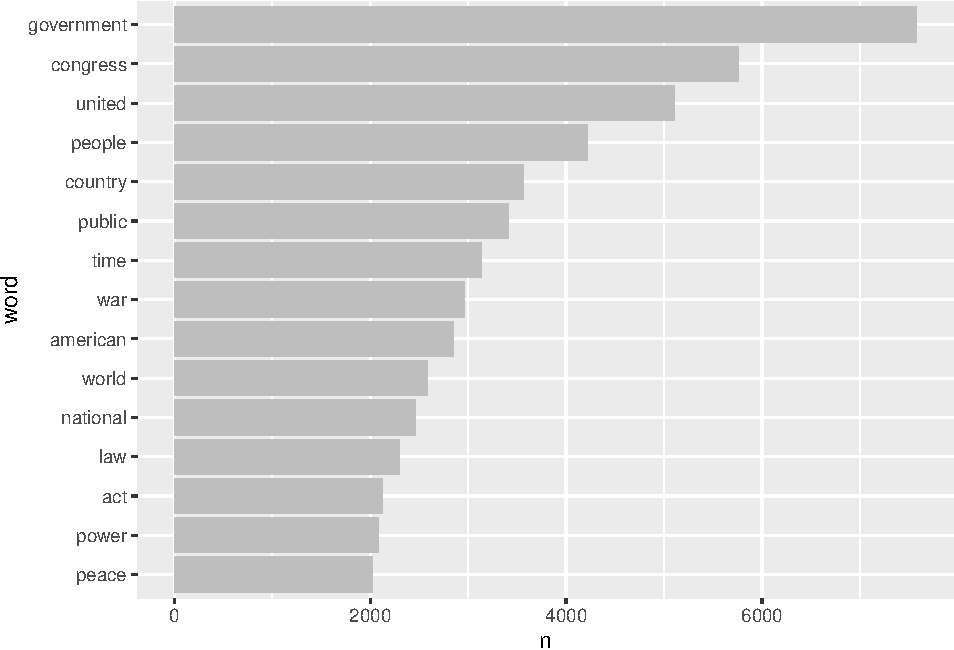
\includegraphics{R-text-analysis_files/figure-latex/word-freq-plot-1.pdf}

Now let's look at a different question: In any given year, how often is the word `peace' used and how often is the word `war' used?

\begin{Shaded}
\begin{Highlighting}[]
\CommentTok{\# steps:}
\CommentTok{\# Select only the words \textquotesingle{}war\textquotesingle{} and \textquotesingle{}peace\textquotesingle{}.}
\CommentTok{\# count ocurrences of each per year}

\NormalTok{tidy\_sotu\_words }\SpecialCharTok{\%\textgreater{}\%}
  \FunctionTok{filter}\NormalTok{(word }\SpecialCharTok{\%in\%} \FunctionTok{c}\NormalTok{(}\StringTok{"war"}\NormalTok{, }\StringTok{"peace"}\NormalTok{)) }\SpecialCharTok{\%\textgreater{}\%} 
  \FunctionTok{count}\NormalTok{(year, word)}
\end{Highlighting}
\end{Shaded}

\begin{verbatim}
#> # A tibble: 442 x 3
#>     year word      n
#>    <int> <chr> <int>
#>  1  1790 peace     3
#>  2  1790 war       4
#>  3  1791 peace     4
#>  4  1791 war       1
#>  5  1792 peace     5
#>  6  1792 war       2
#>  7  1793 peace     6
#>  8  1793 war       4
#>  9  1794 peace     3
#> 10  1794 war       1
#> # ... with 432 more rows
\end{verbatim}

Now we can plot this as a bar chart that shows for each year the proportion of each of these two words out of the total of how often both words are used.

\begin{Shaded}
\begin{Highlighting}[]
\CommentTok{\# plot n by year, and use position \textquotesingle{}fill\textquotesingle{} to show the proportion}

\NormalTok{tidy\_sotu\_words }\SpecialCharTok{\%\textgreater{}\%}
  \FunctionTok{filter}\NormalTok{(word }\SpecialCharTok{\%in\%} \FunctionTok{c}\NormalTok{(}\StringTok{"war"}\NormalTok{, }\StringTok{"peace"}\NormalTok{)) }\SpecialCharTok{\%\textgreater{}\%} 
  \FunctionTok{count}\NormalTok{(year, word) }\SpecialCharTok{\%\textgreater{}\%} 
  \FunctionTok{ggplot}\NormalTok{(}\FunctionTok{aes}\NormalTok{(year, n, }\AttributeTok{fill =}\NormalTok{ word)) }\SpecialCharTok{+}
    \FunctionTok{geom\_col}\NormalTok{(}\AttributeTok{position =} \StringTok{"fill"}\NormalTok{)}
\end{Highlighting}
\end{Shaded}

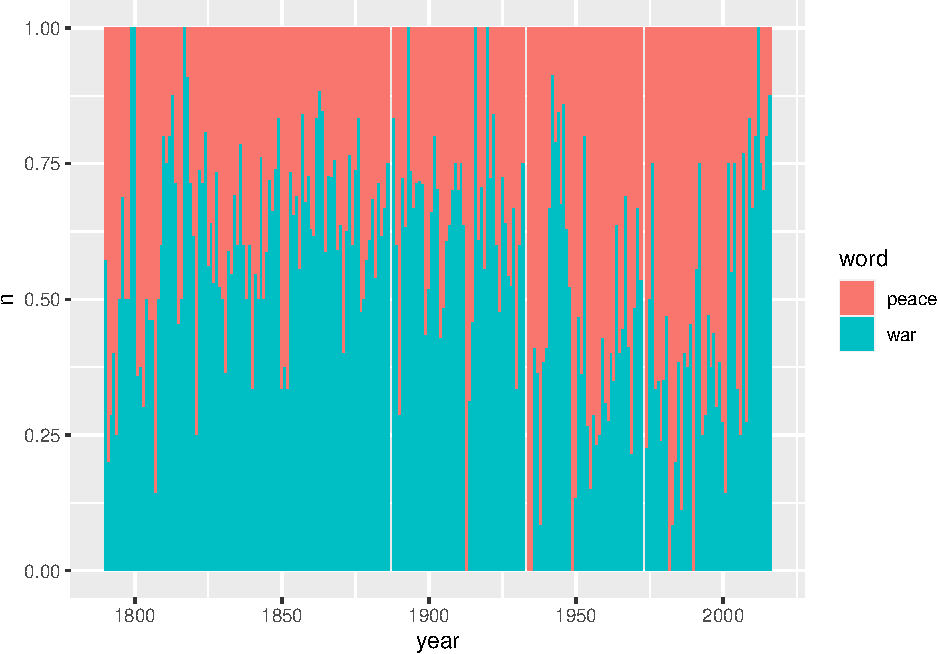
\includegraphics{R-text-analysis_files/figure-latex/plot-word-years-1.pdf}

As another example let us calculate the average number of words per speech for each president: How long was the average speech of each president and who are the most `wordy' presidents?

First we summarize the words per president per speech:

\begin{Shaded}
\begin{Highlighting}[]
\NormalTok{tidy\_sotu\_words }\SpecialCharTok{\%\textgreater{}\%}
  \FunctionTok{count}\NormalTok{(president, doc\_id)}
\end{Highlighting}
\end{Shaded}

\begin{verbatim}
#> # A tibble: 240 x 3
#>    president       doc_id                       n
#>    <chr>           <chr>                    <int>
#>  1 Abraham Lincoln abraham-lincoln-1861.txt  2578
#>  2 Abraham Lincoln abraham-lincoln-1862.txt  3088
#>  3 Abraham Lincoln abraham-lincoln-1863.txt  2398
#>  4 Abraham Lincoln abraham-lincoln-1864.txt  2398
#>  5 Andrew Jackson  andrew-jackson-1829.txt   3849
#>  6 Andrew Jackson  andrew-jackson-1830.txt   5428
#>  7 Andrew Jackson  andrew-jackson-1831.txt   2612
#>  8 Andrew Jackson  andrew-jackson-1832.txt   2881
#>  9 Andrew Jackson  andrew-jackson-1833.txt   2869
#> 10 Andrew Jackson  andrew-jackson-1834.txt   4952
#> # ... with 230 more rows
\end{verbatim}

Then we use the output table and group it by president. That allows us to calculate the average number of words per speech.

\begin{Shaded}
\begin{Highlighting}[]
\NormalTok{tidy\_sotu\_words }\SpecialCharTok{\%\textgreater{}\%}
  \FunctionTok{count}\NormalTok{(president, doc\_id)  }\SpecialCharTok{\%\textgreater{}\%} 
  \FunctionTok{group\_by}\NormalTok{(president) }\SpecialCharTok{\%\textgreater{}\%} 
  \FunctionTok{summarize}\NormalTok{(}\AttributeTok{avg\_words =} \FunctionTok{mean}\NormalTok{(n)) }\SpecialCharTok{\%\textgreater{}\%} 
  \FunctionTok{arrange}\NormalTok{(}\FunctionTok{desc}\NormalTok{(avg\_words))}
\end{Highlighting}
\end{Shaded}

\begin{verbatim}
#> # A tibble: 42 x 2
#>    president           avg_words
#>    <chr>                   <dbl>
#>  1 William Howard Taft     9126.
#>  2 William McKinley        7797 
#>  3 Jimmy Carter            7673.
#>  4 Theodore Roosevelt      7356 
#>  5 James K. Polk           6920.
#>  6 Grover Cleveland        5736.
#>  7 James Buchanan          5409 
#>  8 Benjamin Harrison       5308.
#>  9 Rutherford B. Hayes     4411 
#> 10 Martin Van Buren        4286.
#> # ... with 32 more rows
\end{verbatim}

\hypertarget{term-frequency}{%
\section{Term frequency}\label{term-frequency}}

Often a raw count of a word is less important than understanding how often that word appears \emph{relative to the total number} of words in a text. This ratio is called the \textbf{term frequency}. We can use \texttt{dplyr} to calculate it like this:

\begin{Shaded}
\begin{Highlighting}[]
\NormalTok{tidy\_sotu\_words }\SpecialCharTok{\%\textgreater{}\%}
  \FunctionTok{count}\NormalTok{(doc\_id, word, }\AttributeTok{sort =}\NormalTok{ T)  }\SpecialCharTok{\%\textgreater{}\%}  \CommentTok{\# count occurrence of word and sort descending}
  \FunctionTok{group\_by}\NormalTok{(doc\_id) }\SpecialCharTok{\%\textgreater{}\%} 
  \FunctionTok{mutate}\NormalTok{(}\AttributeTok{n\_tot =} \FunctionTok{sum}\NormalTok{(n),              }\CommentTok{\# count total number of words per doc}
         \AttributeTok{term\_freq =}\NormalTok{ n}\SpecialCharTok{/}\NormalTok{n\_tot)}
\end{Highlighting}
\end{Shaded}

\begin{verbatim}
#> # A tibble: 358,186 x 5
#> # Groups:   doc_id [240]
#>    doc_id                       word               n n_tot term_freq
#>    <chr>                        <chr>          <int> <int>     <dbl>
#>  1 harry-s-truman-1946.txt      dollars          207 12614   0.0164 
#>  2 jimmy-carter-1980b.txt       congress         204 16128   0.0126 
#>  3 harry-s-truman-1946.txt      war              201 12614   0.0159 
#>  4 william-howard-taft-1910.txt government       164 11178   0.0147 
#>  5 james-k-polk-1846.txt        mexico           158  7023   0.0225 
#>  6 richard-m-nixon-1974b.txt    federal          141  9996   0.0141 
#>  7 harry-s-truman-1946.txt      million          138 12614   0.0109 
#>  8 harry-s-truman-1946.txt      fiscal           129 12614   0.0102 
#>  9 jimmy-carter-1981.txt        administration   129 16595   0.00777
#> 10 william-howard-taft-1912.txt government       129 10215   0.0126 
#> # ... with 358,176 more rows
\end{verbatim}

Let's plot the distribution of the term frequency for the speeches:

\begin{Shaded}
\begin{Highlighting}[]
\NormalTok{tidy\_sotu\_words }\SpecialCharTok{\%\textgreater{}\%}
  \FunctionTok{count}\NormalTok{(doc\_id, word)  }\SpecialCharTok{\%\textgreater{}\%}  \CommentTok{\# count n for each word}
  \FunctionTok{group\_by}\NormalTok{(doc\_id) }\SpecialCharTok{\%\textgreater{}\%} 
  \FunctionTok{mutate}\NormalTok{(}\AttributeTok{n\_tot =} \FunctionTok{sum}\NormalTok{(n), }\CommentTok{\# count total number of words per doc}
         \AttributeTok{term\_freq =}\NormalTok{ n}\SpecialCharTok{/}\NormalTok{n\_tot) }\SpecialCharTok{\%\textgreater{}\%} 
  \FunctionTok{ggplot}\NormalTok{(}\FunctionTok{aes}\NormalTok{(term\_freq)) }\SpecialCharTok{+}
    \FunctionTok{geom\_histogram}\NormalTok{() }
\end{Highlighting}
\end{Shaded}

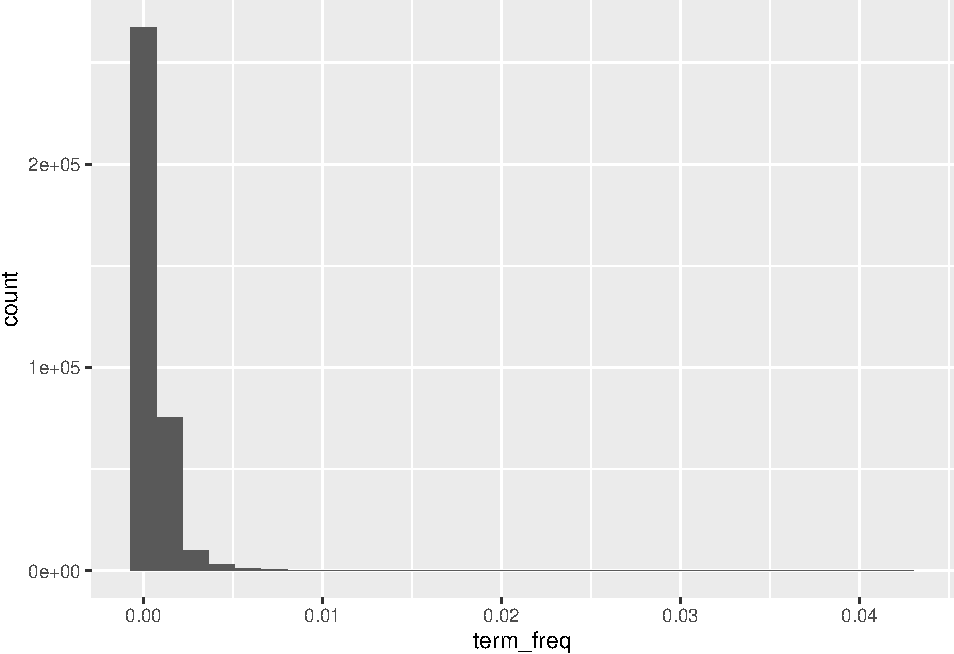
\includegraphics{R-text-analysis_files/figure-latex/termfreq-plot-1.pdf}

This distribution makes sense. Many words are used relatively rarely in a text. Only a few have a high term frequency.

Assuming that terms with high relative frequency are an indicator of significance we can find the term with the highest term frequency for each president:

\begin{Shaded}
\begin{Highlighting}[]
\NormalTok{tidy\_sotu\_words }\SpecialCharTok{\%\textgreater{}\%}
  \FunctionTok{count}\NormalTok{(president, word)  }\SpecialCharTok{\%\textgreater{}\%}  \CommentTok{\# count n for each word}
  \FunctionTok{group\_by}\NormalTok{(president) }\SpecialCharTok{\%\textgreater{}\%} 
  \FunctionTok{mutate}\NormalTok{(}\AttributeTok{n\_tot =} \FunctionTok{sum}\NormalTok{(n), }\CommentTok{\# count total number of words per doc}
         \AttributeTok{term\_freq =}\NormalTok{ n}\SpecialCharTok{/}\NormalTok{n\_tot) }\SpecialCharTok{\%\textgreater{}\%} 
  \FunctionTok{arrange}\NormalTok{(}\FunctionTok{desc}\NormalTok{(term\_freq)) }\SpecialCharTok{\%\textgreater{}\%} \CommentTok{\# sort by term frequency}
  \FunctionTok{top\_n}\NormalTok{(}\DecValTok{1}\NormalTok{) }\SpecialCharTok{\%\textgreater{}\%}  \CommentTok{\# take the top for each president}
  \FunctionTok{print}\NormalTok{(}\AttributeTok{n =} \ConstantTok{Inf}\NormalTok{) }\CommentTok{\# print all rows}
\end{Highlighting}
\end{Shaded}

\begin{verbatim}
#> # A tibble: 44 x 5
#> # Groups:   president [42]
#>    president             word           n n_tot term_freq
#>    <chr>                 <chr>      <int> <int>     <dbl>
#>  1 John Adams            united        49  2768   0.0177 
#>  2 John Tyler            government   209 12596   0.0166 
#>  3 Martin Van Buren      government   256 17145   0.0149 
#>  4 William J. Clinton    people       336 22713   0.0148 
#>  5 Franklin D. Roosevelt war          283 19311   0.0147 
#>  6 William McKinley      government   452 31188   0.0145 
#>  7 Andrew Jackson        government   436 31031   0.0141 
#>  8 Donald Trump          american     135  9690   0.0139 
#>  9 Andrew Johnson        government   207 14968   0.0138 
#> 10 George Washington     united        86  6226   0.0138 
#> 11 Calvin Coolidge       government   274 20518   0.0134 
#> 12 James K. Polk         mexico       360 27679   0.0130 
#> 13 James Buchanan        government   279 21636   0.0129 
#> 14 Zachary Taylor        congress      38  2948   0.0129 
#> 15 Ulysses S. Grant      united       359 27933   0.0129 
#> 16 William Howard Taft   government   461 36506   0.0126 
#> 17 Grover Cleveland      government   574 45889   0.0125 
#> 18 Franklin Pierce       united       200 16240   0.0123 
#> 19 George Bush           world         82  6706   0.0122 
#> 20 James Monroe          united       184 15157   0.0121 
#> 21 George W. Bush        america      209 17265   0.0121 
#> 22 Millard Fillmore      government   135 11986   0.0113 
#> 23 John Quincy Adams     congress     131 11788   0.0111 
#> 24 Harry S Truman        war          308 27819   0.0111 
#> 25 Gerald R. Ford        federal       65  5879   0.0111 
#> 26 Herbert Hoover        government   121 10947   0.0111 
#> 27 Rutherford B. Hayes   congress     194 17644   0.0110 
#> 28 Chester A. Arthur     government   185 16961   0.0109 
#> 29 Lyndon B. Johnson     congress     115 11207   0.0103 
#> 30 James Madison         war           85  8327   0.0102 
#> 31 Barack Obama          america      204 20529   0.00994
#> 32 Benjamin Harrison     government   209 21230   0.00984
#> 33 Richard M. Nixon      federal      232 23701   0.00979
#> 34 Jimmy Carter          congress     518 53710   0.00964
#> 35 John F. Kennedy       world         68  7302   0.00931
#> 36 Theodore Roosevelt    government   528 58848   0.00897
#> 37 Ronald Reagan         government   133 15005   0.00886
#> 38 Ronald Reagan         people       133 15005   0.00886
#> 39 Woodrow Wilson        government   105 11982   0.00876
#> 40 Warren G. Harding     public        39  4583   0.00851
#> 41 Dwight D. Eisenhower  world        204 24410   0.00836
#> 42 Thomas Jefferson      country       58  7418   0.00782
#> 43 Abraham Lincoln       congress      81 10462   0.00774
#> 44 Abraham Lincoln       united        81 10462   0.00774
\end{verbatim}

\begin{quote}
\begin{quote}
\begin{quote}
CHALLENGE: Pick one president. For each of his speeches, which is the term with highest term frequency? Create a table as output. (Hint: \texttt{top\_n}might be useful)
\end{quote}
\end{quote}
\end{quote}

\hypertarget{tf-idf}{%
\section{Tf-idf}\label{tf-idf}}

So far we've been looking at term frequency per document. What if we want to know about words that seem more important based on the contents of the \emph{entire} corpus?

For this, we can use \textbf{term-frequency according to inverse document frequency}, also callled \textbf{tf-idf}. Tf-idf measures how important a word is within a corpus by scaling term frequency per document according to the inverse of the term's document frequency (number of documents within the corpus in which the term appears divided by the number of documents).

The tf-idf value will be:

\begin{itemize}
\tightlist
\item
  lower for words that appear frequently in many documents of the corpus, and lowest when the word occurs in virtually all documents.
\item
  higher for words that appear frequently in just a few documents of the corpus, this lending high discriminatory power to those few documents.
\end{itemize}

The intuition here is that if a term appears frequently in a document, we think that it is important but if that word appears in too many other documents, it is not that unique and thus perhaps not that important.

The \texttt{tidytext} package includes a function \texttt{bind\_tf\_idf}. It takes a table that contains one-row-per-term-per-document, the name of the column that contains the words (terms), the name of the column which contains the doc-id, and the name of the column that contains the document-term counts.

So below we aggregate our tibble with the word tokens to create the one-row-per-term-per-document table and then pipe it into the \texttt{bind\_tf\_idf} function.

\begin{Shaded}
\begin{Highlighting}[]
\NormalTok{tidy\_sotu\_words }\SpecialCharTok{\%\textgreater{}\%}
  \FunctionTok{count}\NormalTok{(doc\_id, word, }\AttributeTok{sort =} \ConstantTok{TRUE}\NormalTok{)  }\SpecialCharTok{\%\textgreater{}\%}  \CommentTok{\# aggregate to count n for each word}
  \FunctionTok{bind\_tf\_idf}\NormalTok{(word, doc\_id, n) }
\end{Highlighting}
\end{Shaded}

\begin{verbatim}
#> # A tibble: 358,186 x 6
#>    doc_id                       word               n      tf     idf    tf_idf
#>    <chr>                        <chr>          <int>   <dbl>   <dbl>     <dbl>
#>  1 harry-s-truman-1946.txt      dollars          207 0.0164  0.598   0.00981  
#>  2 jimmy-carter-1980b.txt       congress         204 0.0126  0.00418 0.0000528
#>  3 harry-s-truman-1946.txt      war              201 0.0159  0.0339  0.000540 
#>  4 william-howard-taft-1910.txt government       164 0.0147  0.00418 0.0000613
#>  5 james-k-polk-1846.txt        mexico           158 0.0225  0.799   0.0180   
#>  6 richard-m-nixon-1974b.txt    federal          141 0.0141  0.293   0.00414  
#>  7 harry-s-truman-1946.txt      million          138 0.0109  0.710   0.00777  
#>  8 harry-s-truman-1946.txt      fiscal           129 0.0102  0.511   0.00522  
#>  9 jimmy-carter-1981.txt        administration   129 0.00777 0.277   0.00215  
#> 10 william-howard-taft-1912.txt government       129 0.0126  0.00418 0.0000527
#> # ... with 358,176 more rows
\end{verbatim}

Our function added three columns to the aggregated table which contain term frequency (\texttt{tf}), inverse document frequency (\texttt{idf}) and Tf-idf (\texttt{tf\_idf}).

Let's look at some of the words in the corpus that have the highest tf-idf scores, which means words that are particularly distinctive for their documents.

\begin{Shaded}
\begin{Highlighting}[]
\NormalTok{tidy\_sotu\_words }\SpecialCharTok{\%\textgreater{}\%}
  \FunctionTok{count}\NormalTok{(doc\_id, word, }\AttributeTok{sort =} \ConstantTok{TRUE}\NormalTok{)  }\SpecialCharTok{\%\textgreater{}\%} 
  \FunctionTok{bind\_tf\_idf}\NormalTok{(word, doc\_id, n) }\SpecialCharTok{\%\textgreater{}\%} 
  \FunctionTok{arrange}\NormalTok{(}\FunctionTok{desc}\NormalTok{(tf\_idf))}
\end{Highlighting}
\end{Shaded}

\begin{verbatim}
#> # A tibble: 358,186 x 6
#>    doc_id                        word          n      tf   idf tf_idf
#>    <chr>                         <chr>     <int>   <dbl> <dbl>  <dbl>
#>  1 donald-trump-2019.txt         applause    104 0.0424   2.22 0.0942
#>  2 lyndon-b-johnson-1966.txt     vietnam      32 0.0152   2.35 0.0356
#>  3 jimmy-carter-1980a.txt        soviet       31 0.0218   1.49 0.0325
#>  4 george-w-bush-2003.txt        hussein      19 0.00811  3.87 0.0314
#>  5 george-w-bush-2003.txt        saddam       19 0.00811  3.69 0.0299
#>  6 franklin-d-roosevelt-1943.txt 1942         13 0.00758  3.87 0.0294
#>  7 dwight-d-eisenhower-1961.txt  1953         23 0.00747  3.87 0.0289
#>  8 john-adams-1800.txt           gentlemen     8 0.0153   1.77 0.0270
#>  9 benjamin-harrison-1892.txt    1892         40 0.00741  3.53 0.0262
#> 10 franklin-d-roosevelt-1942.txt hitler        7 0.00527  4.79 0.0252
#> # ... with 358,176 more rows
\end{verbatim}

To understand the occurrence of the years as being particularly distinctive we might need to look more closely at the speeches themselves, and determine whether the years are significant or whether they need to be removed from the text either permanently in the clean up or temporarily using \texttt{filter()}.

\begin{quote}
\begin{quote}
\begin{quote}
CHALLENGE: Pick the same president you chose above. For each of his speeches, which is the term with highest tf-idf? Create a table as output. (Hint: Remember to group by doc\_id before you use top\_n)
\end{quote}
\end{quote}
\end{quote}

\hypertarget{n-grams}{%
\section{N-Grams}\label{n-grams}}

We mentioned n-grams in the intro, but let's revisit them here and take a look at the most common bigrams in the speeches. Remember we can use the \texttt{unnest\_token()} function on our texts and explicitly tell it to generate bigrams:

\begin{Shaded}
\begin{Highlighting}[]
\NormalTok{sotu\_whole }\SpecialCharTok{\%\textgreater{}\%}
  \FunctionTok{unnest\_tokens}\NormalTok{(bigram, text, }\AttributeTok{token =} \StringTok{"ngrams"}\NormalTok{, }\AttributeTok{n =} \DecValTok{2}\NormalTok{) }\CommentTok{\# create bigram}
\end{Highlighting}
\end{Shaded}

\begin{verbatim}
#> # A tibble: 1,987,963 x 8
#>        X president        year years_active party      sotu_type doc_id   bigram
#>    <int> <chr>           <int> <chr>        <chr>      <chr>     <chr>    <chr> 
#>  1    73 Abraham Lincoln  1861 1861-1865    Republican written   abraham~ fello~
#>  2    73 Abraham Lincoln  1861 1861-1865    Republican written   abraham~ citiz~
#>  3    73 Abraham Lincoln  1861 1861-1865    Republican written   abraham~ of the
#>  4    73 Abraham Lincoln  1861 1861-1865    Republican written   abraham~ the s~
#>  5    73 Abraham Lincoln  1861 1861-1865    Republican written   abraham~ senat~
#>  6    73 Abraham Lincoln  1861 1861-1865    Republican written   abraham~ and h~
#>  7    73 Abraham Lincoln  1861 1861-1865    Republican written   abraham~ house~
#>  8    73 Abraham Lincoln  1861 1861-1865    Republican written   abraham~ of re~
#>  9    73 Abraham Lincoln  1861 1861-1865    Republican written   abraham~ repre~
#> 10    73 Abraham Lincoln  1861 1861-1865    Republican written   abraham~ in the
#> # ... with 1,987,953 more rows
\end{verbatim}

Let's see the most common bigrams:

\begin{Shaded}
\begin{Highlighting}[]
\NormalTok{sotu\_whole }\SpecialCharTok{\%\textgreater{}\%}
  \FunctionTok{unnest\_tokens}\NormalTok{(bigram, text, }\AttributeTok{token =} \StringTok{"ngrams"}\NormalTok{, }\AttributeTok{n =} \DecValTok{2}\NormalTok{) }\SpecialCharTok{\%\textgreater{}\%} 
  \FunctionTok{count}\NormalTok{(bigram, }\AttributeTok{sort =} \ConstantTok{TRUE}\NormalTok{) }\CommentTok{\# count occurrences and sort descending}
\end{Highlighting}
\end{Shaded}

\begin{verbatim}
#> # A tibble: 475,240 x 2
#>    bigram            n
#>    <chr>         <int>
#>  1 of the        33699
#>  2 in the        12608
#>  3 to the        11684
#>  4 for the        6926
#>  5 and the        6265
#>  6 by the         5625
#>  7 of our         5219
#>  8 the united     4816
#>  9 united states  4808
#> 10 it is          4774
#> # ... with 475,230 more rows
\end{verbatim}

Ok, so we again need to remove the stopwords. First let us separate the two words into two columns ``word1'' and ``word2'' with \texttt{separate} from the \texttt{tidyr} package:

\begin{Shaded}
\begin{Highlighting}[]
\NormalTok{sotu\_whole }\SpecialCharTok{\%\textgreater{}\%}
  \FunctionTok{unnest\_tokens}\NormalTok{(bigram, text, }\AttributeTok{token =} \StringTok{"ngrams"}\NormalTok{, }\AttributeTok{n =} \DecValTok{2}\NormalTok{) }\SpecialCharTok{\%\textgreater{}\%} 
  \FunctionTok{separate}\NormalTok{(bigram, }\FunctionTok{c}\NormalTok{(}\StringTok{"word1"}\NormalTok{, }\StringTok{"word2"}\NormalTok{), }\AttributeTok{sep =} \StringTok{" "}\NormalTok{)}
\end{Highlighting}
\end{Shaded}

\begin{verbatim}
#> # A tibble: 1,987,963 x 9
#>        X president        year years_active party     sotu_~1 doc_id word1 word2
#>    <int> <chr>           <int> <chr>        <chr>     <chr>   <chr>  <chr> <chr>
#>  1    73 Abraham Lincoln  1861 1861-1865    Republic~ written abrah~ fell~ citi~
#>  2    73 Abraham Lincoln  1861 1861-1865    Republic~ written abrah~ citi~ of   
#>  3    73 Abraham Lincoln  1861 1861-1865    Republic~ written abrah~ of    the  
#>  4    73 Abraham Lincoln  1861 1861-1865    Republic~ written abrah~ the   sena~
#>  5    73 Abraham Lincoln  1861 1861-1865    Republic~ written abrah~ sena~ and  
#>  6    73 Abraham Lincoln  1861 1861-1865    Republic~ written abrah~ and   house
#>  7    73 Abraham Lincoln  1861 1861-1865    Republic~ written abrah~ house of   
#>  8    73 Abraham Lincoln  1861 1861-1865    Republic~ written abrah~ of    repr~
#>  9    73 Abraham Lincoln  1861 1861-1865    Republic~ written abrah~ repr~ in   
#> 10    73 Abraham Lincoln  1861 1861-1865    Republic~ written abrah~ in    the  
#> # ... with 1,987,953 more rows, and abbreviated variable name 1: sotu_type
\end{verbatim}

Now we use dplyr's \texttt{filter()} function to select only the words in each column that are not in the stopwords.

\begin{Shaded}
\begin{Highlighting}[]
\NormalTok{sotu\_whole }\SpecialCharTok{\%\textgreater{}\%}
  \FunctionTok{unnest\_tokens}\NormalTok{(bigram, text, }\AttributeTok{token =} \StringTok{"ngrams"}\NormalTok{, }\AttributeTok{n =} \DecValTok{2}\NormalTok{) }\SpecialCharTok{\%\textgreater{}\%} 
  \FunctionTok{separate}\NormalTok{(bigram, }\FunctionTok{c}\NormalTok{(}\StringTok{"word1"}\NormalTok{, }\StringTok{"word2"}\NormalTok{), }\AttributeTok{sep =} \StringTok{" "}\NormalTok{) }\SpecialCharTok{\%\textgreater{}\%} \CommentTok{\# separate into cols}
  \FunctionTok{filter}\NormalTok{(}\SpecialCharTok{!}\NormalTok{word1 }\SpecialCharTok{\%in\%}\NormalTok{ stop\_words}\SpecialCharTok{$}\NormalTok{word, }\CommentTok{\# remove stopwords}
         \SpecialCharTok{!}\NormalTok{word2 }\SpecialCharTok{\%in\%}\NormalTok{ stop\_words}\SpecialCharTok{$}\NormalTok{word)}
\end{Highlighting}
\end{Shaded}

\begin{verbatim}
#> # A tibble: 219,471 x 9
#>        X president        year years_active party     sotu_~1 doc_id word1 word2
#>    <int> <chr>           <int> <chr>        <chr>     <chr>   <chr>  <chr> <chr>
#>  1    73 Abraham Lincoln  1861 1861-1865    Republic~ written abrah~ fell~ citi~
#>  2    73 Abraham Lincoln  1861 1861-1865    Republic~ written abrah~ unpr~ poli~
#>  3    73 Abraham Lincoln  1861 1861-1865    Republic~ written abrah~ poli~ trou~
#>  4    73 Abraham Lincoln  1861 1861-1865    Republic~ written abrah~ abun~ harv~
#>  5    73 Abraham Lincoln  1861 1861-1865    Republic~ written abrah~ pecu~ exig~
#>  6    73 Abraham Lincoln  1861 1861-1865    Republic~ written abrah~ fore~ nati~
#>  7    73 Abraham Lincoln  1861 1861-1865    Republic~ written abrah~ prof~ soli~
#>  8    73 Abraham Lincoln  1861 1861-1865    Republic~ written abrah~ soli~ chie~
#>  9    73 Abraham Lincoln  1861 1861-1865    Republic~ written abrah~ dome~ affa~
#> 10    73 Abraham Lincoln  1861 1861-1865    Republic~ written abrah~ disl~ port~
#> # ... with 219,461 more rows, and abbreviated variable name 1: sotu_type
\end{verbatim}

Lastly, we re-unite the two word columns into back into our bigrams and save it into a new table \texttt{sotu\_bigrams}.

\begin{Shaded}
\begin{Highlighting}[]
\NormalTok{sotu\_bigrams }\OtherTok{\textless{}{-}}\NormalTok{ sotu\_whole }\SpecialCharTok{\%\textgreater{}\%}
  \FunctionTok{unnest\_tokens}\NormalTok{(bigram, text, }\AttributeTok{token =} \StringTok{"ngrams"}\NormalTok{, }\AttributeTok{n =} \DecValTok{2}\NormalTok{) }\SpecialCharTok{\%\textgreater{}\%} 
  \FunctionTok{separate}\NormalTok{(bigram, }\FunctionTok{c}\NormalTok{(}\StringTok{"word1"}\NormalTok{, }\StringTok{"word2"}\NormalTok{), }\AttributeTok{sep =} \StringTok{" "}\NormalTok{) }\SpecialCharTok{\%\textgreater{}\%} \CommentTok{\# separate into cols}
  \FunctionTok{filter}\NormalTok{(}\SpecialCharTok{!}\NormalTok{word1 }\SpecialCharTok{\%in\%}\NormalTok{ stop\_words}\SpecialCharTok{$}\NormalTok{word, }\CommentTok{\# remove stopwords}
         \SpecialCharTok{!}\NormalTok{word2 }\SpecialCharTok{\%in\%}\NormalTok{ stop\_words}\SpecialCharTok{$}\NormalTok{word) }\SpecialCharTok{\%\textgreater{}\%} 
  \FunctionTok{unite}\NormalTok{(bigram, word1, word2, }\AttributeTok{sep =} \StringTok{" "}\NormalTok{)  }\CommentTok{\# combine columns}


\NormalTok{sotu\_bigrams }\SpecialCharTok{\%\textgreater{}\%} 
  \FunctionTok{count}\NormalTok{(bigram, }\AttributeTok{sort =} \ConstantTok{TRUE}\NormalTok{)}
\end{Highlighting}
\end{Shaded}

\begin{verbatim}
#> # A tibble: 131,899 x 2
#>    bigram                 n
#>    <chr>              <int>
#>  1 federal government   479
#>  2 american people      439
#>  3 june 30              325
#>  4 fellow citizens      299
#>  5 public debt          283
#>  6 public lands         256
#>  7 health care          253
#>  8 social security      233
#>  9 post office          202
#> 10 annual message       200
#> # ... with 131,889 more rows
\end{verbatim}

A bigram can also be treated as a term in a document in the same way that we treated individual words. That means we can look at tf-idf values in the same way. For example, we can find out the most distinct bigrams that the presidents uttered in all their respective speeches taken together.

We count per president and bigram and then bind the tf-idf value with the \texttt{bind\_tf\_idf} function. In order to get the top bigram for each president we then group by president, and sort and retrieve the highest value for each.

\begin{Shaded}
\begin{Highlighting}[]
\NormalTok{sotu\_bigrams }\SpecialCharTok{\%\textgreater{}\%}
  \FunctionTok{count}\NormalTok{(president, bigram) }\SpecialCharTok{\%\textgreater{}\%}
  \FunctionTok{bind\_tf\_idf}\NormalTok{(bigram, president, n) }\SpecialCharTok{\%\textgreater{}\%}
  \FunctionTok{group\_by}\NormalTok{(president) }\SpecialCharTok{\%\textgreater{}\%}  
  \FunctionTok{arrange}\NormalTok{(}\FunctionTok{desc}\NormalTok{(tf\_idf)) }\SpecialCharTok{\%\textgreater{}\%} 
  \FunctionTok{top\_n}\NormalTok{(}\DecValTok{1}\NormalTok{)}
\end{Highlighting}
\end{Shaded}

\begin{verbatim}
#> # A tibble: 45 x 6
#> # Groups:   president [42]
#>    president          bigram              n      tf   idf tf_idf
#>    <chr>              <chr>           <int>   <dbl> <dbl>  <dbl>
#>  1 John Adams         john adams          3 0.00510 3.74  0.0191
#>  2 George W. Bush     al qaida           35 0.00628 2.64  0.0166
#>  3 Thomas Jefferson   gun boats           7 0.00462 3.04  0.0141
#>  4 Thomas Jefferson   port towns          7 0.00462 3.04  0.0141
#>  5 Thomas Jefferson   sea port            7 0.00462 3.04  0.0141
#>  6 William J. Clinton 21st century       59 0.00830 1.66  0.0138
#>  7 Zachary Taylor     german empire       5 0.00789 1.66  0.0131
#>  8 Lyndon B. Johnson  south vietnam      13 0.00424 3.04  0.0129
#>  9 James Madison      james madison       8 0.00412 3.04  0.0125
#> 10 Harry S Truman     million dollars   119 0.0129  0.965 0.0124
#> # ... with 35 more rows
\end{verbatim}

\begin{quote}
\begin{quote}
\begin{quote}
CHALLENGE: Again, pick the same president you chose above. For each of his speeches, which is the bigram with highest tf-idf? Create a table as output.
\end{quote}
\end{quote}
\end{quote}

\hypertarget{co-occurrence}{%
\section{Co-occurrence}\label{co-occurrence}}

Co-occurrences give us a sense of words that appear in the same text, but not necessarily next to each other.

For this section we will make use of the \texttt{widyr} package. The function which helps us do this is the \texttt{pairwise\_count()} function. It lets us count common pairs of words co-appearing within the same speech.

Behind the scenes, this function first turns our table into a wide matrix. In our case that matrix will be made up of the individual words and the cell values will be the counts of in how many speeches they co-occur, like this:

\begin{verbatim}
#>      we thus have
#> we   NA    4    5
#> thus  4   NA    2
#> have  5    2   NA
\end{verbatim}

It then will turn the matrix back into a tidy form, where each row contains the word pairs and the count of their co-occurrence. Since we don't care about the order of the words, we will not count the upper triangle of the wide matrix, which leaves us with:

\begin{verbatim}
#>             
#>    we thus 4
#>    we have 5
#>  thus have 2
\end{verbatim}

Since processing the entire corpus would take too long here, we will only look at the last 100 words of each speech: which words occur most commonly together at the end of the speeches?

\begin{Shaded}
\begin{Highlighting}[]
\FunctionTok{library}\NormalTok{(widyr)}

\NormalTok{sotu\_word\_pairs }\OtherTok{\textless{}{-}}\NormalTok{ sotu\_whole }\SpecialCharTok{\%\textgreater{}\%} 
  \FunctionTok{mutate}\NormalTok{(}\AttributeTok{speech\_end =} \FunctionTok{word}\NormalTok{(text, }\SpecialCharTok{{-}}\DecValTok{100}\NormalTok{, }\AttributeTok{end =} \SpecialCharTok{{-}}\DecValTok{1}\NormalTok{)) }\SpecialCharTok{\%\textgreater{}\%}  \CommentTok{\# extract last 100 words}
  \FunctionTok{unnest\_tokens}\NormalTok{(word, speech\_end) }\SpecialCharTok{\%\textgreater{}\%}   \CommentTok{\# tokenize}
  \FunctionTok{filter}\NormalTok{(}\SpecialCharTok{!}\NormalTok{word }\SpecialCharTok{\%in\%}\NormalTok{ stop\_words}\SpecialCharTok{$}\NormalTok{word) }\SpecialCharTok{\%\textgreater{}\%}  \CommentTok{\# remove stopwords}
  \FunctionTok{pairwise\_count}\NormalTok{(word, doc\_id, }\AttributeTok{sort =} \ConstantTok{TRUE}\NormalTok{, }\AttributeTok{upper =} \ConstantTok{FALSE}\NormalTok{) }\CommentTok{\# don\textquotesingle{}t include upper triangle of matrix}

\NormalTok{sotu\_word\_pairs}
\end{Highlighting}
\end{Shaded}

\begin{verbatim}
#> # A tibble: 126,853 x 3
#>    item1      item2       n
#>    <chr>      <chr>   <dbl>
#>  1 god        bless      41
#>  2 god        america    39
#>  3 bless      america    34
#>  4 people     country    27
#>  5 god        nation     24
#>  6 world      god        23
#>  7 god        people     23
#>  8 god        country    22
#>  9 people     america    22
#> 10 government people     21
#> # ... with 126,843 more rows
\end{verbatim}

To visualize the co-occurrence network of words that occur together at the end of 10 or more speeches, we use the \texttt{igraph} package to convert our table into a network graph and the \texttt{ggraph} package which adds functionality to ggplot to make it easier to plot a network.

\begin{Shaded}
\begin{Highlighting}[]
\FunctionTok{library}\NormalTok{(igraph)}
\FunctionTok{library}\NormalTok{(ggraph)}

\NormalTok{sotu\_word\_pairs }\SpecialCharTok{\%\textgreater{}\%} 
  \FunctionTok{filter}\NormalTok{(n }\SpecialCharTok{\textgreater{}=} \DecValTok{10}\NormalTok{) }\SpecialCharTok{\%\textgreater{}\%}  \CommentTok{\# only word pairs that occur 10 or more times}
  \FunctionTok{graph\_from\_data\_frame}\NormalTok{() }\SpecialCharTok{\%\textgreater{}\%} \CommentTok{\#convert to graph}
  \FunctionTok{ggraph}\NormalTok{(}\AttributeTok{layout =} \StringTok{"fr"}\NormalTok{) }\SpecialCharTok{+} \CommentTok{\# place nodes according to the force{-}directed algorithm of Fruchterman and Reingold}
  \FunctionTok{geom\_edge\_link}\NormalTok{(}\FunctionTok{aes}\NormalTok{(}\AttributeTok{edge\_alpha =}\NormalTok{ n, }\AttributeTok{edge\_width =}\NormalTok{ n), }\AttributeTok{edge\_colour =} \StringTok{"tomato"}\NormalTok{) }\SpecialCharTok{+}
  \FunctionTok{geom\_node\_point}\NormalTok{(}\AttributeTok{size =} \DecValTok{5}\NormalTok{) }\SpecialCharTok{+}
  \FunctionTok{geom\_node\_text}\NormalTok{(}\FunctionTok{aes}\NormalTok{(}\AttributeTok{label =}\NormalTok{ name), }\AttributeTok{repel =} \ConstantTok{TRUE}\NormalTok{, }
                 \AttributeTok{point.padding =} \FunctionTok{unit}\NormalTok{(}\FloatTok{0.2}\NormalTok{, }\StringTok{"lines"}\NormalTok{)) }\SpecialCharTok{+}
  \FunctionTok{theme\_void}\NormalTok{()}
\end{Highlighting}
\end{Shaded}

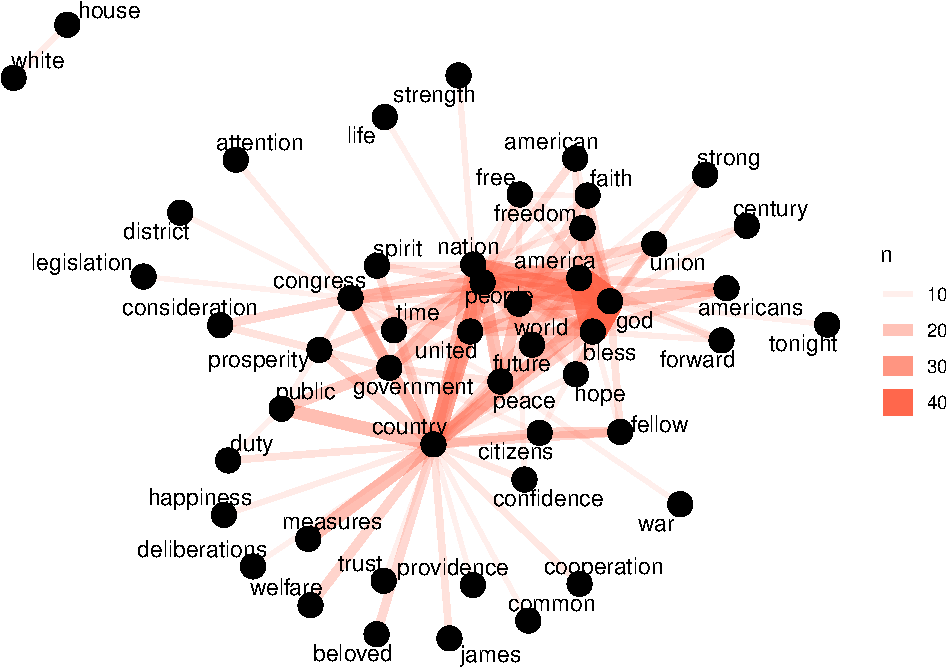
\includegraphics{R-text-analysis_files/figure-latex/plot-network-1.pdf}

There are alternative approaches for this as well. See for example the \texttt{findAssocs} function in the \texttt{tm} package.

\hypertarget{document-term-matrix}{%
\section{Document-Term Matrix}\label{document-term-matrix}}

A \href{https://en.wikipedia.org/wiki/Document-term_matrix}{document-term matrix (DTM)} is a format which is frequently used in text analysis. It is a matrix where we can see the counts of each term per document. In a DTM each row represents a document, each column represents a term, and the cell values are the counts of the occurrences of the term for the particular document.

\texttt{tidytext} provides functionality to convert to and from DTMs, if for example, your analysis requires specific functions from a different R package which only works with DTM object types.

The \texttt{cast\_dtm} function can be used to create a DTM object from a tidy table.

Let's assume that for some reason we want to use the \texttt{findAssoc()} function from the \texttt{tm} package.

First we use dplyr to create a table with the document name, the term, and the count.

\begin{Shaded}
\begin{Highlighting}[]
\CommentTok{\# make a table with document, term, count}
\NormalTok{tidy\_sotu\_words }\SpecialCharTok{\%\textgreater{}\%} 
  \FunctionTok{count}\NormalTok{(doc\_id, word) }
\end{Highlighting}
\end{Shaded}

\begin{verbatim}
#> # A tibble: 358,186 x 3
#>    doc_id                   word               n
#>    <chr>                    <chr>          <int>
#>  1 abraham-lincoln-1861.txt 1,470,018          1
#>  2 abraham-lincoln-1861.txt 1,500              1
#>  3 abraham-lincoln-1861.txt 100,000            1
#>  4 abraham-lincoln-1861.txt 102,532,509.27     1
#>  5 abraham-lincoln-1861.txt 12,528,000         1
#>  6 abraham-lincoln-1861.txt 13,606,759.11      1
#>  7 abraham-lincoln-1861.txt 1830               1
#>  8 abraham-lincoln-1861.txt 1859               1
#>  9 abraham-lincoln-1861.txt 1860               2
#> 10 abraham-lincoln-1861.txt 1861               6
#> # ... with 358,176 more rows
\end{verbatim}

Now we cast it as a DTM.

\begin{Shaded}
\begin{Highlighting}[]
\NormalTok{sotu\_dtm }\OtherTok{\textless{}{-}}\NormalTok{ tidy\_sotu\_words }\SpecialCharTok{\%\textgreater{}\%} 
  \FunctionTok{count}\NormalTok{(doc\_id, word) }\SpecialCharTok{\%\textgreater{}\%} 
  \FunctionTok{cast\_dtm}\NormalTok{(doc\_id, word, n) }

\FunctionTok{class}\NormalTok{(sotu\_dtm)}
\end{Highlighting}
\end{Shaded}

\begin{verbatim}
#> [1] "DocumentTermMatrix"    "simple_triplet_matrix"
\end{verbatim}

Finally, let's use it in the \texttt{tm} package:

\begin{Shaded}
\begin{Highlighting}[]
\FunctionTok{library}\NormalTok{(tm)}

\CommentTok{\# look at the terms with tm function}
\FunctionTok{Terms}\NormalTok{(sotu\_dtm) }\SpecialCharTok{\%\textgreater{}\%} \FunctionTok{tail}\NormalTok{()}
\end{Highlighting}
\end{Shaded}

\begin{verbatim}
#> [1] "queretaro"    "refreshments" "schleswig"    "sedulous"     "subagents"   
#> [6] "transcript"
\end{verbatim}

\begin{Shaded}
\begin{Highlighting}[]
\CommentTok{\# most frequent terms}
\FunctionTok{findFreqTerms}\NormalTok{(sotu\_dtm, }\AttributeTok{lowfreq =} \DecValTok{5000}\NormalTok{)}
\end{Highlighting}
\end{Shaded}

\begin{verbatim}
#> [1] "congress"   "government" "united"
\end{verbatim}

\begin{Shaded}
\begin{Highlighting}[]
\CommentTok{\# find terms associated with "citizen"}
\FunctionTok{findAssocs}\NormalTok{(sotu\_dtm, }\StringTok{"citizen"}\NormalTok{, }\AttributeTok{corlimit =} \FloatTok{0.5}\NormalTok{)}
\end{Highlighting}
\end{Shaded}

\begin{verbatim}
#> $citizen
#>        laws citizenship  protection   contained    entitled  government 
#>        0.62        0.59        0.56        0.54        0.53        0.53 
#>    citizens  postmaster     careful    question      report       suits 
#>        0.52        0.52        0.51        0.51        0.51        0.51
\end{verbatim}

Conversely, \texttt{tidytext} implements the \texttt{tidy} function (originally from the \texttt{broom} package) to import DocumentTermMatrix objects. Note that it only takes the cells from the DTM that are not 0, so there will be no rows with 0 counts.

\hypertarget{sentiment-analysis}{%
\section{Sentiment analysis}\label{sentiment-analysis}}

\texttt{tidytext} comes with a dataset \texttt{sentiments} which contains several sentiment lexicons, where each word is attributed a certain sentiment, like this:

\begin{Shaded}
\begin{Highlighting}[]
\NormalTok{sentiments}
\end{Highlighting}
\end{Shaded}

\begin{verbatim}
#> # A tibble: 6,786 x 2
#>    word        sentiment
#>    <chr>       <chr>    
#>  1 2-faces     negative 
#>  2 abnormal    negative 
#>  3 abolish     negative 
#>  4 abominable  negative 
#>  5 abominably  negative 
#>  6 abominate   negative 
#>  7 abomination negative 
#>  8 abort       negative 
#>  9 aborted     negative 
#> 10 aborts      negative 
#> # ... with 6,776 more rows
\end{verbatim}

Here we will take a look at how the sentiment of the speeches change over time. We will use the lexicon from \href{https://www.cs.uic.edu/~liub/FBS/sentiment-analysis.html}{Bing Liu and collaborators}, which assigns positive/negative labels for each word:

\begin{Shaded}
\begin{Highlighting}[]
\NormalTok{bing\_lex }\OtherTok{\textless{}{-}} \FunctionTok{get\_sentiments}\NormalTok{(}\StringTok{"bing"}\NormalTok{)}
\NormalTok{bing\_lex}
\end{Highlighting}
\end{Shaded}

\begin{verbatim}
#> # A tibble: 6,786 x 2
#>    word        sentiment
#>    <chr>       <chr>    
#>  1 2-faces     negative 
#>  2 abnormal    negative 
#>  3 abolish     negative 
#>  4 abominable  negative 
#>  5 abominably  negative 
#>  6 abominate   negative 
#>  7 abomination negative 
#>  8 abort       negative 
#>  9 aborted     negative 
#> 10 aborts      negative 
#> # ... with 6,776 more rows
\end{verbatim}

We can use these sentiments attached to each word and join them to the words of our speeches. We will use \texttt{inner\_join} from \texttt{dplyr}. It will take all rows with words from \texttt{tidy\_sotu\_words} that match words in \texttt{bing\_lex}, eliminating rows where the word cannot be found in the lexicon. Since our columns to join on have the same name (\texttt{word}) we don't need to explicitly name it.

\begin{Shaded}
\begin{Highlighting}[]
\NormalTok{sotu\_sentiments }\OtherTok{\textless{}{-}}\NormalTok{ tidy\_sotu\_words }\SpecialCharTok{\%\textgreater{}\%} 
  \FunctionTok{inner\_join}\NormalTok{(bing\_lex)  }\CommentTok{\# join to add semtinemt column}

\NormalTok{sotu\_sentiments}
\end{Highlighting}
\end{Shaded}

\begin{verbatim}
#> # A tibble: 106,649 x 9
#>        X president        year years_active party   sotu_~1 doc_id word  senti~2
#>    <int> <chr>           <int> <chr>        <chr>   <chr>   <chr>  <chr> <chr>  
#>  1    73 Abraham Lincoln  1861 1861-1865    Republ~ written abrah~ trou~ negati~
#>  2    73 Abraham Lincoln  1861 1861-1865    Republ~ written abrah~ grat~ positi~
#>  3    73 Abraham Lincoln  1861 1861-1865    Republ~ written abrah~ unus~ negati~
#>  4    73 Abraham Lincoln  1861 1861-1865    Republ~ written abrah~ abun~ positi~
#>  5    73 Abraham Lincoln  1861 1861-1865    Republ~ written abrah~ pecu~ negati~
#>  6    73 Abraham Lincoln  1861 1861-1865    Republ~ written abrah~ prof~ positi~
#>  7    73 Abraham Lincoln  1861 1861-1865    Republ~ written abrah~ soli~ negati~
#>  8    73 Abraham Lincoln  1861 1861-1865    Republ~ written abrah~ disl~ negati~
#>  9    73 Abraham Lincoln  1861 1861-1865    Republ~ written abrah~ dest~ negati~
#> 10    73 Abraham Lincoln  1861 1861-1865    Republ~ written abrah~ disr~ negati~
#> # ... with 106,639 more rows, and abbreviated variable names 1: sotu_type,
#> #   2: sentiment
\end{verbatim}

Finally we can visualize the proportion of positive sentiment (out of the total of positive and negative) in US State of the Union Addresses over time like this:

\begin{Shaded}
\begin{Highlighting}[]
\NormalTok{sotu\_sentiments }\SpecialCharTok{\%\textgreater{}\%} 
  \FunctionTok{count}\NormalTok{(year, sentiment) }\SpecialCharTok{\%\textgreater{}\%} \CommentTok{\# count by year and sentiment}
  \FunctionTok{pivot\_wider}\NormalTok{(}\AttributeTok{names\_from =} \StringTok{"sentiment"}\NormalTok{, }\AttributeTok{values\_from =} \StringTok{"n"}\NormalTok{) }\SpecialCharTok{\%\textgreater{}\%} \CommentTok{\# create column for positive}
                                                               \CommentTok{\# and negative sentiment}
  \FunctionTok{mutate}\NormalTok{(}\AttributeTok{positive\_ratio =}\NormalTok{ positive}\SpecialCharTok{/}\NormalTok{(negative }\SpecialCharTok{+}\NormalTok{ positive)) }\SpecialCharTok{\%\textgreater{}\%} \CommentTok{\# calculate positive ratio}
  \CommentTok{\# plot}
  \FunctionTok{ggplot}\NormalTok{(}\FunctionTok{aes}\NormalTok{(year, positive\_ratio)) }\SpecialCharTok{+}
    \FunctionTok{geom\_line}\NormalTok{(}\AttributeTok{color=}\StringTok{"gray"}\NormalTok{) }\SpecialCharTok{+}
    \FunctionTok{geom\_smooth}\NormalTok{(}\AttributeTok{span =} \FloatTok{0.3}\NormalTok{, }\AttributeTok{se =} \ConstantTok{FALSE}\NormalTok{) }\SpecialCharTok{+} \CommentTok{\# smooth for easier viewing}
    \FunctionTok{geom\_hline}\NormalTok{(}\AttributeTok{yintercept =}\NormalTok{ .}\DecValTok{5}\NormalTok{, }\AttributeTok{linetype=}\StringTok{"dotted"}\NormalTok{, }\AttributeTok{color =} \StringTok{"orange"}\NormalTok{, }\AttributeTok{size =} \DecValTok{1}\NormalTok{) }\SpecialCharTok{+} \CommentTok{\# .5 as reference}
    \FunctionTok{scale\_x\_continuous}\NormalTok{(}\AttributeTok{breaks =} \FunctionTok{seq}\NormalTok{(}\DecValTok{1790}\NormalTok{, }\DecValTok{2016}\NormalTok{, }\AttributeTok{by =} \DecValTok{10}\NormalTok{)) }\SpecialCharTok{+}
    \FunctionTok{theme}\NormalTok{(}\AttributeTok{axis.text.x =} \FunctionTok{element\_text}\NormalTok{(}\AttributeTok{angle =} \DecValTok{45}\NormalTok{, }\AttributeTok{hjust =} \DecValTok{1}\NormalTok{))}
\end{Highlighting}
\end{Shaded}

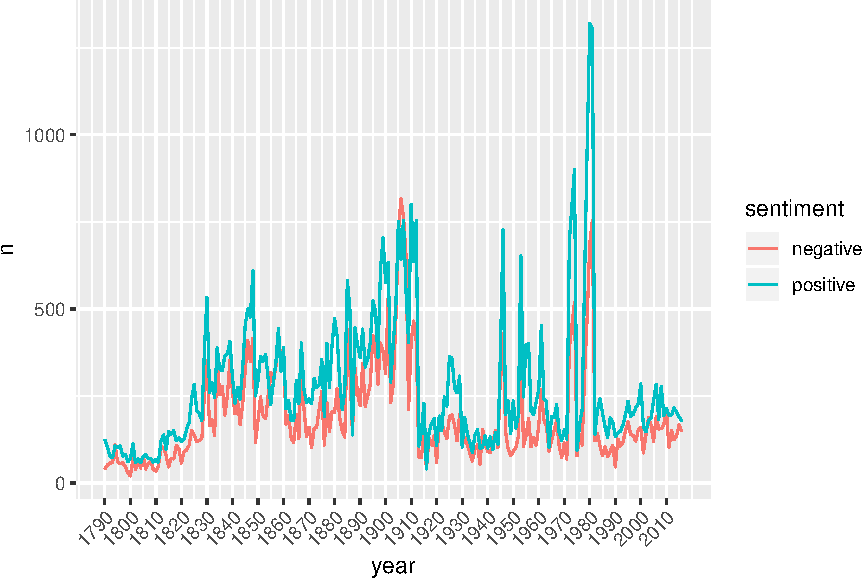
\includegraphics{R-text-analysis_files/figure-latex/sentiment-plot-1.pdf}

  \bibliography{book.bib,packages.bib}

\end{document}
